\clearpage
\appendix

\section{Per-Cell Results}
\label{app:cells}


LongBench categories: Single-Doc QA (NarrativeQA, Qasper, MultiFieldQA-en), Multi-Doc QA (HotpotQA, 2WikiMQA, MuSiQue), Summarization (GovReport, QMSum, Multi-News) and Code (LCC, RepoBench-P); a category's score is the mean over its datasets, each scored on all of its 150--500 samples. RULER uses its 11 subtasks (NIAH-Single-1/2/3, NIAH-MultiKey-1/2/3, NIAH-MultiQuery, NIAH-MultiValue, Common-Words Extraction, Frequent-Words Extraction and Variable Tracking) at 4K context, 500 samples each; the RULER score is the mean over the 11 subtasks.

Tables~\ref{tab:app-cells} and~\ref{tab:app-cells-ruler} (Llama-3-8B-Instruct, LongBench and RULER) and Tables~\ref{tab:app-cells-mistral} and~\ref{tab:app-cells-mistral-ruler} (Mistral-7B-Instruct-v0.2) list every evaluated (task, method, budget) cell on full data. For each task they give three rows: uniform allocation, the rescaled Stage 2 winner (Winner, Stage 3) and NAS-refined, the best configuration of the Stage 4 search. MOSAIC's final configuration is the better of Winner and NAS-refined. Winner rows also cover budgets where Stage 4 did not run, so they give the full winner transfer of Appendix~\ref{app:transfer}.


\begin{table}[t]
  \centering
  \scriptsize
  \setlength{\tabcolsep}{3.5pt}
  \renewcommand{\arraystretch}{0.9}
\begin{tabular}{@{} c l rrrr @{}}
  \toprule
  \textbf{Task} & & \textbf{128} & \textbf{256} & \textbf{512} & \textbf{1024} \\
  \midrule
  \multicolumn{6}{c}{\textbf{SnapKV}} \\
  \midrule
  \multirow{3}{*}{\shortstack[c]{Code\\(430)}} & Uniform & 54.81 & 55.67 & 56.73 & 56.02 \\
   & Winner & 55.86 & \textbf{57.33} & \textbf{58.16} & 58.52 \\
   & NAS-ref. & \textbf{56.09} & 57.31 & 58.01 & \textbf{58.91} \\
  \cmidrule(l){2-6}
  \multirow{3}{*}{\shortstack[c]{Multi-Doc QA\\(274)}} & Uniform & 34.82 & 35.60 & \textbf{35.77} & 35.87 \\
   & Winner & \textbf{35.02} & \textbf{36.31} & 35.73 & \textbf{36.26} \\
   & NAS-ref. & 34.94 & 35.68 & 35.55 & 36.14 \\
  \cmidrule(l){2-6}
  \multirow{3}{*}{\shortstack[c]{Single-Doc QA\\(506)}} & Uniform & 32.97 & \textbf{35.25} & 35.97 & 36.44 \\
   & Winner & 33.51 & 34.51 & \textbf{36.33} & 36.46 \\
   & NAS-ref. & \textbf{33.67} & 34.51 & 35.61 & \textbf{37.01} \\
  \cmidrule(l){2-6}
  \multirow{3}{*}{\shortstack[c]{Summarization\\(732)}} & Uniform & 21.03 & 22.30 & 23.44 & 24.85 \\
   & Winner & \textbf{21.15} & \textbf{22.41} & \textbf{23.71} & \textbf{25.10} \\
   & NAS-ref. & 20.95 & -- & -- & -- \\
  \midrule
  \multicolumn{6}{c}{\textbf{H2O}} \\
  \midrule
  \multirow{3}{*}{\shortstack[c]{Code\\(2456)}} & Uniform & 45.96 & 49.49 & 52.81 & 56.92 \\
   & Winner & 46.59 & \textbf{50.59} & 54.03 & 56.15 \\
   & NAS-ref. & \textbf{47.13} & 50.31 & \textbf{54.51} & \textbf{57.23} \\
  \cmidrule(l){2-6}
  \multirow{3}{*}{\shortstack[c]{Multi-Doc QA\\(448)}} & Uniform & \textbf{32.57} & 32.45 & 32.98 & 33.54 \\
   & Winner & 32.16 & 32.86 & \textbf{34.33} & 34.38 \\
   & NAS-ref. & 32.01 & \textbf{32.92} & 33.50 & \textbf{34.93} \\
  \cmidrule(l){2-6}
  \multirow{3}{*}{\shortstack[c]{Single-Doc QA\\(518)}} & Uniform & 28.21 & 29.96 & 32.41 & 33.60 \\
   & Winner & \textbf{29.72} & 30.70 & 32.21 & 34.20 \\
   & NAS-ref. & 28.32 & \textbf{30.92} & \textbf{32.80} & \textbf{34.69} \\
  \cmidrule(l){2-6}
  \multirow{3}{*}{\shortstack[c]{Summarization\\(552)}} & Uniform & 21.88 & 23.13 & 24.22 & 24.97 \\
   & Winner & 22.02 & 23.17 & \textbf{24.35} & 25.11 \\
   & NAS-ref. & \textbf{22.31} & \textbf{23.33} & 24.32 & \textbf{25.32} \\
  \midrule
  \multicolumn{6}{c}{\textbf{AdaKV}} \\
  \midrule
  \multirow{3}{*}{\shortstack[c]{Code\\(482)}} & Uniform & 57.30 & 58.19 & 58.70 & -- \\
   & Winner & 56.94 & 58.77 & 59.61 & -- \\
   & NAS-ref. & \textbf{58.28} & \textbf{59.62} & \textbf{60.68} & -- \\
  \cmidrule(l){2-6}
  \multirow{3}{*}{\shortstack[c]{Multi-Doc QA\\(188)}} & Uniform & 34.99 & 35.42 & 36.14 & -- \\
   & Winner & 35.38 & \textbf{36.14} & 35.69 & -- \\
   & NAS-ref. & \textbf{35.96} & 36.05 & \textbf{36.33} & -- \\
  \cmidrule(l){2-6}
  \multirow{3}{*}{\shortstack[c]{Single-Doc QA\\(464)}} & Uniform & 32.83 & 35.08 & \textbf{36.68} & -- \\
   & Winner & 33.16 & 35.33 & 36.45 & -- \\
   & NAS-ref. & \textbf{34.64} & \textbf{35.98} & 36.49 & -- \\
  \midrule
  \multicolumn{6}{c}{\textbf{L2Norm}} \\
  \midrule
  \multirow{3}{*}{\shortstack[c]{Code\\(1410)}} & Uniform & 22.54 & 23.57 & 28.14 & 34.95 \\
   & Winner & 26.20 & 30.46 & 35.55 & \textbf{44.47} \\
   & NAS-ref. & \textbf{27.48} & \textbf{30.69} & \textbf{35.90} & 42.61 \\
  \cmidrule(l){2-6}
  \multirow{3}{*}{\shortstack[c]{Multi-Doc QA\\(2236)}} & Uniform & 9.09 & 13.23 & 22.06 & 28.72 \\
   & Winner & 8.18 & 18.41 & 23.91 & 31.37 \\
   & NAS-ref. & \textbf{9.23} & \textbf{18.64} & \textbf{25.49} & \textbf{32.90} \\
  \cmidrule(l){2-6}
  \multirow{3}{*}{\shortstack[c]{Single-Doc QA\\(2120)}} & Uniform & 10.20 & 13.91 & 18.48 & 24.75 \\
   & Winner & 10.52 & \textbf{14.76} & 20.43 & \textbf{29.21} \\
   & NAS-ref. & \textbf{10.63} & 14.02 & \textbf{21.13} & 28.57 \\
  \cmidrule(l){2-6}
  \multirow{3}{*}{\shortstack[c]{Summarization\\(2518)}} & Uniform & 17.73 & 19.79 & 21.30 & 23.01 \\
   & Winner & 17.86 & \textbf{19.98} & \textbf{21.95} & \textbf{23.57} \\
   & NAS-ref. & \textbf{18.69} & 19.82 & 21.74 & 23.33 \\
  \bottomrule
\end{tabular}
  \caption{\textbf{Full-data results for every evaluated LongBench cell, Llama-3-8B-Instruct.} Per task: uniform, the rescaled Stage 2 winner (Winner) and NAS-refined (best of the Stage 4 search); bold: best in each column. The number under each task is the winner's natural average budget, at which Stage 1 found it. ``--'': not run. MOSAIC's final configuration beats uniform in 50 of 54 cells with a Stage 4 search, and the Winner alone in 48 of 57.}
  \label{tab:app-cells}
\end{table}

\begin{table*}[t]
  \centering
  \scriptsize
  \setlength{\tabcolsep}{9pt}
  \renewcommand{\arraystretch}{0.9}
\begin{tabular}{@{} c l rrrrrrr @{}}
  \toprule
  \textbf{Method} & & \textbf{64} & \textbf{128} & \textbf{256} & \textbf{512} & \textbf{1024} & \textbf{1536} & \textbf{2048} \\
  \midrule
  \multirow{3}{*}{\shortstack[c]{SnapKV\\(1756)}} & Uniform & 34.64 & 51.56 & 68.06 & 78.62 & 85.67 & 88.62 & 92.93 \\
   & Winner & \textbf{44.99} & \textbf{58.37} & \textbf{72.28} & \textbf{81.76} & 91.46 & \textbf{98.35} & \textbf{98.91} \\
   & NAS-ref. & -- & 55.91 & 71.07 & -- & \textbf{93.80} & 96.86 & 98.35 \\
  \midrule
  \multirow{3}{*}{\shortstack[c]{H2O\\(2180)}} & Uniform & 7.23 & 12.19 & \textbf{20.02} & 29.64 & 44.35 & 53.39 & 62.82 \\
   & Winner & \textbf{7.60} & 12.22 & 19.61 & \textbf{32.61} & 53.42 & 70.88 & 88.31 \\
   & NAS-ref. & -- & \textbf{15.39} & -- & -- & \textbf{62.52} & \textbf{86.05} & \textbf{96.14} \\
  \midrule
  \multirow{3}{*}{\shortstack[c]{AdaKV\\(2536)}} & Uniform & 35.80 & 50.87 & 68.02 & 78.22 & 86.87 & 89.75 & 93.90 \\
   & Winner & \textbf{35.97} & 55.32 & 68.74 & 78.50 & 87.09 & 94.76 & 98.17 \\
   & NAS-ref. & -- & \textbf{57.40} & \textbf{72.10} & \textbf{83.08} & \textbf{93.78} & \textbf{97.99} & \textbf{98.65} \\
  \midrule
  \multirow{3}{*}{\shortstack[c]{L2Norm\\(2354)}} & Uniform & -- & 4.63 & 17.74 & 27.17 & 35.59 & 42.28 & 49.70 \\
   & Winner & -- & 10.85 & 20.50 & 28.48 & 37.76 & 51.33 & 61.16 \\
   & NAS-ref. & -- & \textbf{13.68} & \textbf{20.83} & \textbf{29.42} & \textbf{67.03} & \textbf{90.19} & \textbf{97.21} \\
  \bottomrule
\end{tabular}
  \caption{\textbf{Full-data results for every evaluated RULER cell, Llama-3-8B-Instruct.} Layout as in Table~\ref{tab:app-cells}; the number under each method is its winner's natural average budget. ``--'': not run (at B64, Winner and NAS-refined need a per-layer floor below 64). MOSAIC's final configuration beats uniform in 21 of 21 cells with a Stage 4 search, and the Winner alone in 26 of 27.}
  \label{tab:app-cells-ruler}
\end{table*}

\begin{table}[t]
  \centering
  \scriptsize
  \setlength{\tabcolsep}{3.5pt}
  \renewcommand{\arraystretch}{0.9}
\begin{tabular}{@{} c l rrrr @{}}
  \toprule
  \textbf{Task} & & \textbf{128} & \textbf{256} & \textbf{512} & \textbf{1024} \\
  \midrule
  \multicolumn{6}{c}{\textbf{L2Norm}} \\
  \midrule
  \multirow{3}{*}{\shortstack[c]{Code}} & Uniform & 22.45 & 25.58 & 28.68 & 33.22 \\
   & Winner & 24.40 & 27.93 & 31.70 & 37.87 \\
   & NAS-ref. & \textbf{24.89} & \textbf{28.18} & \textbf{32.12} & \textbf{38.18} \\
  \cmidrule(l){2-6}
  \multirow{3}{*}{\shortstack[c]{Multi-Doc QA}} & Uniform & 4.96 & 5.73 & 7.55 & 11.01 \\
   & Winner & 5.11 & 6.10 & 8.96 & 16.18 \\
   & NAS-ref. & \textbf{5.84} & \textbf{7.29} & \textbf{12.96} & \textbf{17.45} \\
  \cmidrule(l){2-6}
  \multirow{3}{*}{\shortstack[c]{Single-Doc QA}} & Uniform & 5.03 & 7.27 & 9.83 & 16.27 \\
   & Winner & \textbf{6.04} & 8.81 & 14.55 & 23.15 \\
   & NAS-ref. & 5.88 & \textbf{8.88} & \textbf{14.66} & \textbf{23.46} \\
  \cmidrule(l){2-6}
  \multirow{3}{*}{\shortstack[c]{Summarization}} & Uniform & 18.02 & 19.61 & 20.89 & 22.48 \\
   & Winner & 18.16 & 19.73 & 21.42 & 23.00 \\
   & NAS-ref. & \textbf{18.81} & \textbf{20.40} & \textbf{21.72} & \textbf{23.41} \\
  \bottomrule
\end{tabular}
  \caption{\textbf{Full-data results for every evaluated LongBench cell, Mistral-7B-Instruct-v0.2} (L2Norm). Layout as in Table~\ref{tab:app-cells}. MOSAIC's final configuration beats uniform in 16 of 16 cells, and the Winner alone in 16 of 16.}
  \label{tab:app-cells-mistral}
\end{table}

\begin{table*}[t]
  \centering
  \scriptsize
  \setlength{\tabcolsep}{9pt}
  \renewcommand{\arraystretch}{0.9}
\begin{tabular}{@{} c l rrrrrr @{}}
  \toprule
  \textbf{Method} & & \textbf{128} & \textbf{256} & \textbf{512} & \textbf{1024} & \textbf{1536} & \textbf{2048} \\
  \midrule
  \multirow{3}{*}{\shortstack[c]{L2Norm}} & Uniform & 0.64 & 4.25 & 11.06 & 22.86 & 27.59 & 30.73 \\
   & Winner & 2.74 & 8.78 & \textbf{19.43} & 25.62 & 37.30 & 62.71 \\
   & NAS-ref. & \textbf{3.32} & \textbf{10.29} & 17.90 & \textbf{29.65} & \textbf{43.23} & \textbf{64.58} \\
  \midrule
  \multirow{3}{*}{\shortstack[c]{SnapKV}} & Uniform & 40.89 & 51.74 & 62.83 & 77.13 & 84.66 & 90.22 \\
   & Winner & 38.69 & 50.64 & 62.27 & 77.15 & 84.40 & 88.07 \\
   & NAS-ref. & \textbf{47.38} & \textbf{65.24} & \textbf{71.28} & \textbf{91.06} & \textbf{95.71} & \textbf{96.66} \\
  \midrule
  \multirow{3}{*}{\shortstack[c]{H2O}} & Uniform & 10.14 & 14.09 & 19.21 & 27.68 & 33.96 & 41.05 \\
   & Winner & 9.61 & 13.67 & 18.57 & 37.13 & 54.44 & 82.93 \\
   & NAS-ref. & \textbf{10.67} & \textbf{14.75} & \textbf{43.01} & \textbf{68.02} & \textbf{85.31} & \textbf{88.63} \\
  \midrule
  \multirow{3}{*}{\shortstack[c]{AdaKV}} & Uniform & 36.33 & 49.02 & 60.93 & 76.71 & 83.60 & 87.56 \\
   & Winner & 34.23 & 47.67 & 61.48 & -- & 83.12 & 86.43 \\
   & NAS-ref. & \textbf{52.61} & \textbf{60.28} & \textbf{73.94} & \textbf{77.08} & \textbf{88.32} & \textbf{91.71} \\
  \bottomrule
\end{tabular}
  \caption{\textbf{Full-data results for every evaluated RULER cell, Mistral-7B-Instruct-v0.2.} Layout as in Table~\ref{tab:app-cells-ruler}. ``--'': not run. MOSAIC's final configuration beats uniform in 24 of 24 cells, and the Winner alone in 11 of 23.}
  \label{tab:app-cells-mistral-ruler}
\end{table*}


\subsection{RULER Subtask Breakdown}
\label{app:ruler}

Table~\ref{tab:app-ruler} breaks each RULER cell into its 11 subtasks (S1--3: niah\_single; MK1--3: niah\_multikey; MQ: multiquery; MV: multivalue; CWE/FWE: common/frequent-word extraction; VT: variable tracking). ``Best'' is the configuration with the highest 11-subtask mean in that cell. Averaged over floor-clean cells (floor 64, plus B1536/B2048), NAS gains concentrate on the hardest needle subtasks: MK3 +31.9, S3 +28.0, S1 +23.8, versus CWE +0.8, FWE +3.5 and VT +5.6. The floor-16 H2O B1024 configuration trades CWE accuracy (98.3$\rightarrow$21.5) for needle retrieval.

\begin{table*}[t]
  \centering
  \scriptsize
  \setlength{\tabcolsep}{2.5pt}
  \begin{tabular}{@{}l r r l r r r r r r r r r r r r r @{}}
    \toprule
    Method & B & Floor & Config & S1 & S2 & S3 & MK1 & MK2 & MK3 & MQ & MV & CWE & FWE & VT & NIAH & All \\
    \midrule
    H2O & 128 & 64 & uniform & 2.8 & 2.8 & 0.0 & 4.8 & 4.6 & 0.0 & 1.8 & 1.8 & 30.3 & 78.9 & 6.4 & 2.3 & 12.2 \\
    H2O & 128 & 64 & NAS-refined & 13.6 & 2.8 & 0.0 & 7.4 & 10.8 & 0.0 & 3.7 & 5.9 & 29.6 & 86.1 & 9.4 & 5.5 & 15.4 \\
     &  &  & $\Delta$ & +10.8 & +0.0 & +0.0 & +2.6 & +6.2 & +0.0 & +1.9 & +4.2 & $-$0.7 & +7.2 & +3.0 & +3.2 & +3.2 \\
    \midrule
    H2O & 1024 & 16 & uniform & 10.2 & 44.2 & 0.0 & 47.0 & 57.6 & 7.6 & 24.8 & 30.4 & 98.3 & 96.3 & 71.6 & 27.7 & 44.4 \\
    H2O & 1024 & 16 & NAS-refined & 96.6 & 92.0 & 63.0 & 80.2 & 75.8 & 1.0 & 62.4 & 63.7 & 21.5 & 77.5 & 54.1 & 66.8 & 62.5 \\
     &  &  & $\Delta$ & +86.4 & +47.8 & +63.0 & +33.2 & +18.2 & $-$6.6 & +37.6 & +33.4 & $-$76.8 & $-$18.8 & $-$17.5 & +39.1 & +18.2 \\
    \midrule
    H2O & 1536 & 16 & uniform & 16.2 & 58.8 & 0.0 & 61.0 & 71.8 & 24.6 & 35.6 & 44.4 & 99.3 & 95.1 & 80.4 & 39.0 & 53.4 \\
    H2O & 1536 & 16 & NAS-refined & 96.2 & 96.8 & 65.0 & 98.0 & 99.4 & 51.6 & 80.8 & 77.6 & 98.5 & 95.7 & 86.9 & 83.2 & 86.0 \\
     &  &  & $\Delta$ & +80.0 & +38.0 & +65.0 & +37.0 & +27.6 & +27.0 & +45.1 & +33.2 & $-$0.8 & +0.6 & +6.5 & +44.1 & +32.7 \\
    \midrule
    H2O & 2048 & 64 & uniform & 24.0 & 79.4 & 0.0 & 70.4 & 83.2 & 48.6 & 47.6 & 58.0 & 99.6 & 95.1 & 85.0 & 51.4 & 62.8 \\
    H2O & 2048 & 64 & NAS-refined & 100.0 & 100.0 & 99.4 & 99.6 & 99.0 & 98.6 & 90.7 & 82.3 & 98.8 & 94.7 & 94.5 & 96.2 & 96.1 \\
     &  &  & $\Delta$ & +76.0 & +20.6 & +99.4 & +29.2 & +15.8 & +50.0 & +43.0 & +24.3 & $-$0.9 & $-$0.4 & +9.4 & +44.8 & +33.3 \\
    \midrule
    SnapKV & 64 & 16 & uniform & 99.8 & 93.4 & 0.0 & 91.2 & 48.0 & 0.0 & 7.9 & 17.0 & 1.8 & 1.3 & 20.6 & 44.7 & 34.6 \\
    SnapKV & 64 & 16 & Winner & 100.0 & 97.2 & 0.0 & 96.6 & 76.4 & 0.0 & 23.4 & 36.0 & 2.9 & 34.9 & 27.4 & 53.7 & 45.0 \\
     &  &  & $\Delta$ & +0.2 & +3.8 & +0.0 & +5.4 & +28.4 & +0.0 & +15.5 & +19.0 & +1.1 & +33.6 & +6.8 & +9.0 & +10.4 \\
    \midrule
    SnapKV & 128 & 64 & uniform & 100.0 & 98.6 & 0.2 & 98.0 & 72.8 & 0.0 & 36.2 & 53.1 & 8.2 & 49.5 & 50.6 & 57.4 & 51.6 \\
    SnapKV & 128 & 64 & Winner & 100.0 & 98.4 & 0.2 & 98.4 & 91.4 & 0.0 & 57.8 & 64.0 & 9.3 & 56.4 & 66.1 & 63.8 & 58.4 \\
     &  &  & $\Delta$ & +0.0 & $-$0.2 & +0.0 & +0.4 & +18.6 & +0.0 & +21.6 & +10.9 & +1.0 & +6.9 & +15.6 & +6.4 & +6.8 \\
    \midrule
    SnapKV & 256 & 64 & uniform & 100.0 & 99.8 & 1.4 & 99.4 & 93.0 & 0.0 & 82.5 & 84.5 & 30.8 & 68.0 & 89.3 & 70.1 & 68.1 \\
    SnapKV & 256 & 64 & Winner & 100.0 & 99.6 & 10.2 & 99.4 & 98.0 & 0.0 & 90.2 & 92.3 & 38.0 & 72.5 & 94.7 & 73.7 & 72.3 \\
     &  &  & $\Delta$ & +0.0 & $-$0.2 & +8.8 & +0.0 & +5.0 & +0.0 & +7.7 & +7.8 & +7.3 & +4.5 & +5.4 & +3.6 & +4.2 \\
    \midrule
    SnapKV & 512 & 16 & uniform & 100.0 & 100.0 & 23.4 & 99.4 & 99.6 & 0.0 & 97.8 & 96.5 & 73.4 & 78.7 & 96.2 & 77.1 & 78.6 \\
    SnapKV & 512 & 16 & Winner & 100.0 & 100.0 & 49.6 & 99.4 & 99.6 & 0.6 & 98.5 & 97.5 & 77.1 & 81.3 & 95.8 & 80.6 & 81.8 \\
     &  &  & $\Delta$ & +0.0 & +0.0 & +26.2 & +0.0 & +0.0 & +0.6 & +0.7 & +1.0 & +3.7 & +2.6 & $-$0.3 & +3.6 & +3.1 \\
    \midrule
    SnapKV & 1024 & 16 & uniform & 100.0 & 100.0 & 64.8 & 99.4 & 99.8 & 0.6 & 99.8 & 98.8 & 96.1 & 84.7 & 98.4 & 82.9 & 85.7 \\
    SnapKV & 1024 & 16 & NAS-refined & 100.0 & 100.0 & 94.2 & 99.2 & 99.6 & 67.8 & 99.3 & 97.8 & 88.2 & 89.8 & 95.9 & 94.7 & 93.8 \\
     &  &  & $\Delta$ & +0.0 & +0.0 & +29.4 & $-$0.2 & $-$0.2 & +67.2 & $-$0.4 & $-$1.0 & $-$8.0 & +5.1 & $-$2.5 & +11.8 & +8.1 \\
    \midrule
    SnapKV & 1536 & 16 & uniform & 100.0 & 100.0 & 83.8 & 99.4 & 100.0 & 6.8 & 100.0 & 98.8 & 99.0 & 88.1 & 98.9 & 86.1 & 88.6 \\
    SnapKV & 1536 & 16 & Winner & 100.0 & 100.0 & 99.4 & 99.4 & 99.8 & 97.2 & 99.8 & 98.8 & 98.3 & 90.9 & 98.4 & 99.3 & 98.4 \\
     &  &  & $\Delta$ & +0.0 & +0.0 & +15.6 & +0.0 & $-$0.2 & +90.4 & $-$0.2 & $-$0.1 & $-$0.7 & +2.7 & $-$0.4 & +13.2 & +9.7 \\
    \midrule
    SnapKV & 2048 & 16 & uniform & 100.0 & 100.0 & 92.8 & 99.4 & 100.0 & 43.0 & 99.9 & 98.9 & 99.6 & 89.4 & 99.2 & 91.8 & 92.9 \\
    SnapKV & 2048 & 16 & Winner & 100.0 & 100.0 & 100.0 & 99.6 & 100.0 & 98.6 & 99.9 & 98.8 & 99.6 & 92.6 & 98.9 & 99.6 & 98.9 \\
     &  &  & $\Delta$ & +0.0 & +0.0 & +7.2 & +0.2 & +0.0 & +55.6 & +0.0 & $-$0.1 & +0.0 & +3.2 & $-$0.4 & +7.9 & +6.0 \\
    \bottomrule
  \end{tabular}
  \caption{\textbf{RULER subtask accuracy (string match, \%), uniform vs.\ best configuration per cell, SnapKV and H2O.}}
  \label{tab:app-ruler}
\end{table*}


Table~\ref{tab:app-ruler-adakv} gives the same breakdown for AdaKV. The pattern matches SnapKV and H2O: the largest gains are on niah\_multikey\_3 at B1024 and above.

\begin{table*}[t]
  \centering
  \scriptsize
  \setlength{\tabcolsep}{2.5pt}
  \begin{tabular}{@{}l r r l r r r r r r r r r r r r r @{}}
    \toprule
    Method & B & Floor & Config & S1 & S2 & S3 & MK1 & MK2 & MK3 & MQ & MV & CWE & FWE & VT & NIAH & All \\
    \midrule
    AdaKV & 64 & 16 & uniform & 99.6 & 92.0 & 0.0 & 91.6 & 51.6 & 0.0 & 8.2 & 26.7 & 4.0 & 0.7 & 19.4 & 46.2 & 35.8 \\
    AdaKV & 64 & 16 & Winner & 99.6 & 92.4 & 0.0 & 91.4 & 37.8 & 0.0 & 13.9 & 31.4 & 4.9 & 0.2 & 24.0 & 45.8 & 36.0 \\
     &  &  & $\Delta$ & +0.0 & +0.4 & +0.0 & $-$0.2 & $-$13.8 & +0.0 & +5.7 & +4.7 & +0.9 & $-$0.5 & +4.6 & $-$0.4 & +0.2 \\
    \midrule
    AdaKV & 128 & 64 & uniform & 99.8 & 97.8 & 0.0 & 97.4 & 68.2 & 0.0 & 44.2 & 65.8 & 15.3 & 16.8 & 54.2 & 59.1 & 50.9 \\
    AdaKV & 128 & 64 & NAS-refined & 100.0 & 98.6 & 0.6 & 98.4 & 80.0 & 0.0 & 59.0 & 75.5 & 14.7 & 43.2 & 61.5 & 64.0 & 57.4 \\
     &  &  & $\Delta$ & +0.2 & +0.8 & +0.6 & +1.0 & +11.8 & +0.0 & +14.8 & +9.7 & $-$0.6 & +26.4 & +7.2 & +4.9 & +6.5 \\
    \midrule
    AdaKV & 256 & 64 & uniform & 100.0 & 99.8 & 4.2 & 98.8 & 84.8 & 0.0 & 89.5 & 90.4 & 28.9 & 68.1 & 83.7 & 70.9 & 68.0 \\
    AdaKV & 256 & 64 & NAS-refined & 100.0 & 100.0 & 10.8 & 99.4 & 94.8 & 0.0 & 93.5 & 96.0 & 39.7 & 70.4 & 88.4 & 74.3 & 72.1 \\
     &  &  & $\Delta$ & +0.0 & +0.2 & +6.6 & +0.6 & +10.0 & +0.0 & +4.1 & +5.6 & +10.7 & +2.3 & +4.7 & +3.4 & +4.1 \\
    \midrule
    AdaKV & 512 & 64 & uniform & 100.0 & 100.0 & 32.6 & 99.6 & 97.4 & 0.0 & 98.5 & 97.3 & 59.0 & 81.9 & 94.2 & 78.2 & 78.2 \\
    AdaKV & 512 & 64 & NAS-refined & 100.0 & 100.0 & 58.8 & 99.4 & 98.2 & 0.0 & 99.6 & 97.8 & 81.0 & 82.4 & 96.6 & 81.7 & 83.1 \\
     &  &  & $\Delta$ & +0.0 & +0.0 & +26.2 & $-$0.2 & +0.8 & +0.0 & +1.1 & +0.4 & +22.0 & +0.5 & +2.5 & +3.5 & +4.9 \\
    \midrule
    AdaKV & 1024 & 16 & uniform & 100.0 & 100.0 & 77.4 & 99.6 & 99.2 & 1.6 & 99.8 & 98.0 & 93.6 & 87.3 & 98.9 & 84.5 & 86.9 \\
    AdaKV & 1024 & 16 & NAS-refined & 100.0 & 100.0 & 96.6 & 99.6 & 99.4 & 74.6 & 97.0 & 96.5 & 86.4 & 86.9 & 94.6 & 95.5 & 93.8 \\
     &  &  & $\Delta$ & +0.0 & +0.0 & +19.2 & +0.0 & +0.2 & +73.0 & $-$2.8 & $-$1.5 & $-$7.2 & $-$0.4 & $-$4.3 & +11.0 & +6.9 \\
    \midrule
    AdaKV & 1536 & 16 & uniform & 100.0 & 100.0 & 91.2 & 99.6 & 100.0 & 10.6 & 99.9 & 98.3 & 98.7 & 89.7 & 99.1 & 87.5 & 89.7 \\
    AdaKV & 1536 & 16 & NAS-refined & 100.0 & 100.0 & 97.8 & 99.6 & 100.0 & 92.8 & 99.8 & 98.8 & 99.2 & 90.8 & 99.1 & 98.6 & 98.0 \\
     &  &  & $\Delta$ & +0.0 & +0.0 & +6.6 & +0.0 & +0.0 & +82.2 & $-$0.1 & +0.5 & +0.4 & +1.1 & +0.0 & +11.1 & +8.2 \\
    \midrule
    AdaKV & 2048 & 16 & uniform & 100.0 & 100.0 & 96.6 & 99.4 & 100.0 & 48.8 & 99.9 & 98.5 & 99.6 & 90.9 & 99.3 & 92.9 & 93.9 \\
    AdaKV & 2048 & 16 & NAS-refined & 100.0 & 100.0 & 99.6 & 99.8 & 100.0 & 97.4 & 99.8 & 98.0 & 99.3 & 91.9 & 99.2 & 99.3 & 98.6 \\
     &  &  & $\Delta$ & +0.0 & +0.0 & +3.0 & +0.4 & +0.0 & +48.6 & $-$0.1 & $-$0.5 & $-$0.3 & +1.1 & $-$0.0 & +6.4 & +4.7 \\
    \bottomrule
  \end{tabular}
  \caption{\textbf{AdaKV RULER subtask accuracy (string match, \%), uniform vs.\ best configuration per cell.} B64 has only the rescaled winner, compared with uniform-64 from Stage 2.}
  \label{tab:app-ruler-adakv}
\end{table*}


Table~\ref{tab:app-ruler-l2norm} gives the breakdown for L2Norm, whose RULER searches all used floor 64.

\begin{table*}[t]
  \centering
  \scriptsize
  \setlength{\tabcolsep}{2.5pt}
  \begin{tabular}{@{}l r l r r r r r r r r r r r r r @{}}
    \toprule
    Method & B & Config & S1 & S2 & S3 & MK1 & MK2 & MK3 & MQ & MV & CWE & FWE & VT & NIAH & All \\
    \midrule
    L2Norm & 128 & uniform & 28.2 & 0.0 & 0.0 & 0.0 & 0.0 & 0.0 & 0.0 & 0.0 & 7.1 & 15.0 & 0.6 & 3.5 & 4.6 \\
    L2Norm & 128 & NAS-refined & 90.8 & 0.0 & 0.0 & 0.0 & 0.0 & 0.0 & 0.0 & 0.0 & 9.0 & 39.2 & 11.6 & 11.3 & 13.7 \\
     &  & $\Delta$ & +62.6 & +0.0 & +0.0 & +0.0 & +0.0 & +0.0 & +0.0 & +0.0 & +1.8 & +24.2 & +10.9 & +7.8 & +9.0 \\
    \midrule
    L2Norm & 256 & uniform & 99.6 & 1.0 & 0.0 & 0.0 & 0.0 & 0.0 & 0.0 & 0.0 & 18.5 & 44.9 & 31.0 & 12.6 & 17.7 \\
    L2Norm & 256 & NAS-refined & 99.0 & 0.4 & 0.0 & 0.0 & 0.0 & 0.0 & 0.0 & 0.1 & 16.0 & 52.9 & 60.8 & 12.4 & 20.8 \\
     &  & $\Delta$ & $-$0.6 & $-$0.6 & +0.0 & +0.0 & +0.0 & +0.0 & +0.0 & +0.1 & $-$2.5 & +7.9 & +29.8 & $-$0.1 & +3.1 \\
    \midrule
    L2Norm & 512 & uniform & 100.0 & 5.6 & 0.0 & 0.4 & 0.2 & 0.0 & 0.1 & 0.1 & 35.9 & 64.2 & 92.4 & 13.3 & 27.2 \\
    L2Norm & 512 & NAS-refined & 100.0 & 20.2 & 0.0 & 1.4 & 0.4 & 0.0 & 0.0 & 0.0 & 44.8 & 63.2 & 93.6 & 15.2 & 29.4 \\
     &  & $\Delta$ & +0.0 & +14.6 & +0.0 & +1.0 & +0.2 & +0.0 & $-$0.1 & $-$0.1 & +8.8 & $-$1.0 & +1.3 & +2.0 & +2.3 \\
    \midrule
    L2Norm & 1024 & uniform & 100.0 & 32.0 & 0.2 & 5.4 & 1.4 & 0.4 & 0.2 & 0.2 & 73.6 & 79.1 & 99.0 & 17.5 & 35.6 \\
    L2Norm & 1024 & NAS-refined & 100.0 & 91.2 & 40.2 & 82.0 & 40.4 & 2.2 & 64.2 & 70.8 & 70.8 & 78.1 & 97.4 & 61.4 & 67.0 \\
     &  & $\Delta$ & +0.0 & +59.2 & +40.0 & +76.6 & +39.0 & +1.8 & +64.0 & +70.5 & $-$2.8 & $-$0.9 & $-$1.6 & +43.9 & +31.4 \\
    \midrule
    L2Norm & 1536 & uniform & 100.0 & 64.0 & 0.0 & 16.4 & 2.0 & 1.4 & 2.1 & 2.8 & 92.8 & 84.4 & 99.2 & 23.6 & 42.3 \\
    L2Norm & 1536 & NAS-refined & 100.0 & 99.6 & 97.2 & 97.4 & 92.4 & 42.4 & 88.6 & 95.2 & 95.7 & 85.1 & 98.4 & 89.1 & 90.2 \\
     &  & $\Delta$ & +0.0 & +35.6 & +97.2 & +81.0 & +90.4 & +41.0 & +86.4 & +92.4 & +2.9 & +0.7 & $-$0.8 & +65.5 & +47.9 \\
    \midrule
    L2Norm & 2048 & uniform & 100.0 & 87.0 & 1.4 & 38.4 & 3.8 & 5.8 & 12.1 & 13.2 & 97.9 & 87.8 & 99.2 & 32.7 & 49.7 \\
    L2Norm & 2048 & NAS-refined & 100.0 & 99.8 & 100.0 & 99.0 & 98.2 & 95.2 & 96.6 & 96.5 & 97.3 & 87.3 & 99.3 & 98.2 & 97.2 \\
     &  & $\Delta$ & +0.0 & +12.8 & +98.6 & +60.6 & +94.4 & +89.4 & +84.5 & +83.3 & $-$0.7 & $-$0.5 & +0.1 & +65.5 & +47.5 \\
    \bottomrule
  \end{tabular}
  \caption{\textbf{L2Norm RULER subtask accuracy (string match, \%), uniform vs.\ best configuration per cell} (floor 64).}
  \label{tab:app-ruler-l2norm}
\end{table*}


Tables~\ref{tab:app-ruler-mistral} and~\ref{tab:app-ruler-mistral-2} give the breakdown for Mistral-7B-Instruct-v0.2.

\begin{table*}[tp]
  \centering
  \scriptsize
  \setlength{\tabcolsep}{2.5pt}
  \begin{tabular}{@{}l r l r r r r r r r r r r r r r @{}}
    \toprule
    Method & B & Config & S1 & S2 & S3 & MK1 & MK2 & MK3 & MQ & MV & CWE & FWE & VT & NIAH & All \\
    \midrule
    L2Norm & 128 & uniform & 0.0 & 0.0 & 0.0 & 0.0 & 0.0 & 0.0 & 0.0 & 0.0 & 0.3 & 6.7 & 0.0 & 0.0 & 0.6 \\
     &  & NAS-refined & 0.2 & 0.0 & 0.0 & 0.0 & 0.0 & 0.0 & 0.0 & 0.0 & 0.2 & 36.1 & 0.0 & 0.0 & 3.3 \\
     &  & $\Delta$ & +0.2 & +0.0 & +0.0 & +0.0 & +0.0 & +0.0 & +0.0 & +0.0 & $-$0.1 & +29.5 & +0.0 & +0.0 & +2.7 \\
    \midrule
    L2Norm & 256 & uniform & 0.2 & 0.0 & 0.0 & 0.0 & 0.0 & 0.0 & 0.0 & 0.0 & 1.5 & 44.9 & 0.0 & 0.0 & 4.2 \\
     &  & NAS-refined & 53.0 & 0.0 & 0.0 & 0.0 & 0.0 & 0.0 & 0.0 & 0.0 & 0.5 & 47.4 & 12.4 & 6.6 & 10.3 \\
     &  & $\Delta$ & +52.8 & +0.0 & +0.0 & +0.0 & +0.0 & +0.0 & +0.0 & +0.0 & $-$1.1 & +2.5 & +12.3 & +6.6 & +6.0 \\
    \midrule
    L2Norm & 512 & uniform & 41.0 & 0.0 & 0.0 & 0.0 & 0.0 & 0.0 & 0.0 & 0.0 & 7.2 & 65.8 & 7.6 & 5.1 & 11.1 \\
     &  & Winner & 85.0 & 0.0 & 0.0 & 0.0 & 0.2 & 0.0 & 0.0 & 0.0 & 6.7 & 69.3 & 52.4 & 10.7 & 19.4 \\
     &  & $\Delta$ & +44.0 & +0.0 & +0.0 & +0.0 & +0.2 & +0.0 & +0.0 & +0.0 & $-$0.5 & +3.5 & +44.8 & +5.5 & +8.4 \\
    \midrule
    L2Norm & 1024 & uniform & 79.8 & 0.0 & 0.0 & 0.0 & 0.0 & 0.0 & 0.0 & 0.0 & 18.1 & 77.5 & 76.0 & 10.0 & 22.9 \\
     &  & NAS-refined & 100.0 & 41.2 & 3.4 & 12.2 & 9.0 & 6.6 & 3.6 & 2.7 & 9.5 & 72.5 & 65.5 & 22.3 & 29.7 \\
     &  & $\Delta$ & +20.2 & +41.2 & +3.4 & +12.2 & +9.0 & +6.6 & +3.6 & +2.7 & $-$8.7 & $-$4.9 & $-$10.6 & +12.4 & +6.8 \\
    \midrule
    L2Norm & 1536 & uniform & 94.4 & 0.6 & 0.0 & 0.2 & 0.8 & 0.0 & 0.0 & 0.0 & 32.7 & 83.1 & 91.7 & 12.0 & 27.6 \\
     &  & NAS-refined & 95.4 & 84.0 & 6.6 & 53.2 & 7.6 & 0.8 & 23.6 & 23.6 & 27.1 & 77.3 & 76.3 & 36.9 & 43.2 \\
     &  & $\Delta$ & +1.0 & +83.4 & +6.6 & +53.0 & +6.8 & +0.8 & +23.6 & +23.6 & $-$5.5 & $-$5.8 & $-$15.4 & +24.9 & +15.6 \\
    \midrule
    L2Norm & 2048 & uniform & 97.6 & 0.8 & 0.0 & 0.0 & 2.0 & 1.0 & 0.0 & 0.0 & 54.8 & 85.9 & 96.0 & 12.7 & 30.7 \\
     &  & NAS-refined & 100.0 & 80.6 & 68.6 & 61.8 & 20.2 & 76.8 & 41.2 & 46.8 & 35.0 & 87.1 & 92.2 & 62.0 & 64.6 \\
     &  & $\Delta$ & +2.4 & +79.8 & +68.6 & +61.8 & +18.2 & +75.8 & +41.2 & +46.8 & $-$19.8 & +1.2 & $-$3.8 & +49.3 & +33.8 \\
    \midrule
    SnapKV & 128 & uniform & 96.8 & 83.0 & 0.0 & 80.4 & 69.0 & 0.0 & 4.7 & 5.2 & 8.8 & 61.3 & 40.6 & 42.4 & 40.9 \\
     &  & NAS-refined & 99.2 & 87.8 & 0.2 & 87.8 & 67.0 & 0.0 & 20.9 & 17.4 & 13.8 & 71.9 & 55.3 & 47.5 & 47.4 \\
     &  & $\Delta$ & +2.4 & +4.8 & +0.2 & +7.4 & $-$2.0 & +0.0 & +16.2 & +12.2 & +4.9 & +10.6 & +14.7 & +5.1 & +6.5 \\
    \midrule
    SnapKV & 256 & uniform & 100.0 & 90.4 & 1.4 & 90.6 & 86.6 & 0.0 & 14.8 & 12.9 & 24.1 & 78.9 & 69.3 & 49.6 & 51.7 \\
     &  & NAS-refined & 99.6 & 97.4 & 34.4 & 95.2 & 94.6 & 0.2 & 61.1 & 56.9 & 20.5 & 74.1 & 83.6 & 67.4 & 65.2 \\
     &  & $\Delta$ & $-$0.4 & +7.0 & +33.0 & +4.6 & +8.0 & +0.2 & +46.3 & +43.9 & $-$3.6 & $-$4.7 & +14.3 & +17.8 & +13.5 \\
    \midrule
    SnapKV & 512 & uniform & 100.0 & 95.4 & 16.8 & 94.2 & 94.4 & 0.0 & 38.9 & 25.6 & 50.3 & 85.8 & 89.7 & 58.2 & 62.8 \\
     &  & NAS-refined & 100.0 & 95.0 & 58.8 & 96.8 & 94.2 & 0.6 & 68.5 & 61.8 & 48.9 & 74.3 & 85.2 & 72.0 & 71.3 \\
     &  & $\Delta$ & +0.0 & $-$0.4 & +42.0 & +2.6 & $-$0.2 & +0.6 & +29.6 & +36.1 & $-$1.3 & $-$11.5 & $-$4.5 & +13.8 & +8.4 \\
    \midrule
    SnapKV & 1024 & uniform & 100.0 & 97.8 & 57.0 & 97.0 & 99.2 & 0.0 & 74.9 & 58.4 & 77.6 & 89.5 & 97.0 & 73.0 & 77.1 \\
     &  & NAS-refined & 100.0 & 99.8 & 97.2 & 97.8 & 99.8 & 74.4 & 96.3 & 91.2 & 63.0 & 88.5 & 93.6 & 94.6 & 91.1 \\
     &  & $\Delta$ & +0.0 & +2.0 & +40.2 & +0.8 & +0.6 & +74.4 & +21.4 & +32.9 & $-$14.6 & $-$1.0 & $-$3.5 & +21.5 & +13.9 \\
    \midrule
    SnapKV & 1536 & uniform & 100.0 & 99.0 & 82.0 & 97.2 & 99.6 & 8.8 & 88.5 & 80.8 & 86.7 & 90.3 & 98.2 & 82.0 & 84.7 \\
     &  & NAS-refined & 100.0 & 99.8 & 100.0 & 97.6 & 99.6 & 90.6 & 98.5 & 94.1 & 83.0 & 91.1 & 98.5 & 97.5 & 95.7 \\
     &  & $\Delta$ & +0.0 & +0.8 & +18.0 & +0.4 & +0.0 & +81.8 & +10.0 & +13.2 & $-$3.7 & +0.8 & +0.2 & +15.5 & +11.1 \\
    \midrule
    SnapKV & 2048 & uniform & 100.0 & 99.4 & 92.4 & 97.6 & 99.8 & 37.4 & 94.3 & 90.5 & 91.1 & 91.1 & 98.9 & 88.9 & 90.2 \\
     &  & NAS-refined & 100.0 & 99.8 & 97.6 & 97.4 & 99.8 & 91.6 & 98.9 & 97.1 & 90.7 & 91.3 & 99.0 & 97.8 & 96.7 \\
     &  & $\Delta$ & +0.0 & +0.4 & +5.2 & $-$0.2 & +0.0 & +54.2 & +4.6 & +6.6 & $-$0.3 & +0.2 & +0.2 & +8.8 & +6.4 \\
    \bottomrule
  \end{tabular}
  \caption{\textbf{Mistral-7B-Instruct-v0.2 RULER subtask accuracy (string match, \%), uniform vs.\ best configuration per cell, L2Norm and SnapKV.}}
  \label{tab:app-ruler-mistral}
\end{table*}

\begin{table*}[tp]
  \centering
  \scriptsize
  \setlength{\tabcolsep}{2.5pt}
  \begin{tabular}{@{}l r l r r r r r r r r r r r r r @{}}
    \toprule
    Method & B & Config & S1 & S2 & S3 & MK1 & MK2 & MK3 & MQ & MV & CWE & FWE & VT & NIAH & All \\
    \midrule
    H2O & 128 & uniform & 0.0 & 0.0 & 0.0 & 0.0 & 1.0 & 0.0 & 0.0 & 0.0 & 26.9 & 76.5 & 7.2 & 0.1 & 10.1 \\
     &  & NAS-refined & 0.0 & 0.0 & 0.0 & 0.0 & 1.2 & 0.0 & 0.0 & 0.1 & 31.6 & 75.1 & 9.4 & 0.2 & 10.7 \\
     &  & $\Delta$ & +0.0 & +0.0 & +0.0 & +0.0 & +0.2 & +0.0 & +0.0 & +0.1 & +4.7 & $-$1.3 & +2.2 & +0.0 & +0.5 \\
    \midrule
    H2O & 256 & uniform & 0.0 & 0.0 & 0.0 & 0.2 & 3.4 & 0.0 & 0.1 & 0.1 & 55.0 & 83.9 & 12.3 & 0.5 & 14.1 \\
     &  & NAS-refined & 0.0 & 0.0 & 0.0 & 0.8 & 5.6 & 0.0 & 0.1 & 0.3 & 57.2 & 83.9 & 14.4 & 0.8 & 14.8 \\
     &  & $\Delta$ & +0.0 & +0.0 & +0.0 & +0.6 & +2.2 & +0.0 & +0.0 & +0.2 & +2.2 & $-$0.1 & +2.1 & +0.4 & +0.7 \\
    \midrule
    H2O & 512 & uniform & 0.4 & 0.4 & 0.0 & 3.0 & 11.0 & 0.2 & 0.6 & 0.8 & 75.2 & 90.5 & 29.2 & 2.1 & 19.2 \\
     &  & NAS-refined & 54.6 & 79.0 & 0.2 & 58.2 & 66.8 & 3.0 & 19.6 & 20.2 & 57.1 & 85.4 & 28.9 & 37.7 & 43.0 \\
     &  & $\Delta$ & +54.2 & +78.6 & +0.2 & +55.2 & +55.8 & +2.8 & +19.0 & +19.3 & $-$18.0 & $-$5.1 & $-$0.2 & +35.6 & +23.8 \\
    \midrule
    H2O & 1024 & uniform & 2.8 & 2.0 & 0.0 & 9.8 & 27.8 & 3.4 & 4.5 & 6.7 & 88.4 & 92.1 & 67.0 & 7.1 & 27.7 \\
     &  & NAS-refined & 97.8 & 81.0 & 63.0 & 69.6 & 77.2 & 57.8 & 37.8 & 38.1 & 73.7 & 90.9 & 61.4 & 65.3 & 68.0 \\
     &  & $\Delta$ & +95.0 & +79.0 & +63.0 & +59.8 & +49.4 & +54.4 & +33.3 & +31.5 & $-$14.7 & $-$1.3 & $-$5.6 & +58.2 & +40.3 \\
    \midrule
    H2O & 1536 & uniform & 3.8 & 7.8 & 0.0 & 17.4 & 41.6 & 12.6 & 10.9 & 14.6 & 92.1 & 92.7 & 80.0 & 13.6 & 34.0 \\
     &  & NAS-refined & 98.0 & 94.0 & 70.4 & 88.8 & 89.0 & 88.4 & 74.8 & 66.0 & 90.8 & 92.3 & 86.0 & 83.7 & 85.3 \\
     &  & $\Delta$ & +94.2 & +86.2 & +70.4 & +71.4 & +47.4 & +75.8 & +63.8 & +51.4 & $-$1.3 & $-$0.4 & +6.0 & +70.1 & +51.4 \\
    \midrule
    H2O & 2048 & uniform & 9.6 & 19.4 & 0.0 & 28.0 & 54.0 & 27.4 & 18.8 & 23.4 & 93.7 & 92.9 & 84.4 & 22.6 & 41.1 \\
     &  & NAS-refined & 100.0 & 98.4 & 72.8 & 84.8 & 88.6 & 92.8 & 81.2 & 73.7 & 94.0 & 93.0 & 95.7 & 86.5 & 88.6 \\
     &  & $\Delta$ & +90.4 & +79.0 & +72.8 & +56.8 & +34.6 & +65.4 & +62.5 & +50.3 & +0.2 & +0.1 & +11.3 & +64.0 & +47.6 \\
    \midrule
    AdaKV & 128 & uniform & 79.8 & 77.2 & 0.0 & 70.8 & 77.2 & 0.0 & 2.4 & 4.2 & 11.4 & 45.4 & 31.3 & 38.9 & 36.3 \\
     &  & NAS-refined & 89.8 & 90.8 & 0.4 & 90.8 & 84.8 & 0.0 & 35.4 & 38.2 & 13.5 & 65.7 & 69.4 & 53.8 & 52.6 \\
     &  & $\Delta$ & +10.0 & +13.6 & +0.4 & +20.0 & +7.6 & +0.0 & +33.0 & +34.1 & +2.1 & +20.3 & +38.1 & +14.8 & +16.3 \\
    \midrule
    AdaKV & 256 & uniform & 97.2 & 90.4 & 0.4 & 91.0 & 91.0 & 0.0 & 8.5 & 12.2 & 19.2 & 76.5 & 52.8 & 48.8 & 49.0 \\
     &  & NAS-refined & 99.8 & 92.0 & 11.4 & 91.0 & 87.6 & 0.0 & 57.2 & 51.0 & 17.8 & 81.1 & 74.2 & 61.3 & 60.3 \\
     &  & $\Delta$ & +2.6 & +1.6 & +11.0 & +0.0 & $-$3.4 & +0.0 & +48.8 & +38.8 & $-$1.5 & +4.7 & +21.4 & +12.4 & +11.3 \\
    \midrule
    AdaKV & 512 & uniform & 100.0 & 95.2 & 14.2 & 95.2 & 95.6 & 0.0 & 35.5 & 32.2 & 35.3 & 85.9 & 81.1 & 58.5 & 60.9 \\
     &  & NAS-refined & 99.4 & 97.2 & 80.0 & 96.2 & 95.2 & 0.2 & 83.1 & 70.8 & 25.1 & 77.5 & 88.6 & 77.8 & 73.9 \\
     &  & $\Delta$ & $-$0.6 & +2.0 & +65.8 & +1.0 & $-$0.4 & +0.2 & +47.6 & +38.5 & $-$10.2 & $-$8.4 & +7.5 & +19.3 & +13.0 \\
    \midrule
    AdaKV & 1024 & uniform & 100.0 & 98.0 & 63.4 & 97.0 & 97.6 & 0.0 & 76.0 & 65.8 & 62.0 & 88.2 & 95.7 & 74.7 & 76.7 \\
     &  & NAS-refined & 100.0 & 99.0 & 48.6 & 97.4 & 98.6 & 0.0 & 84.2 & 80.9 & 54.5 & 88.1 & 96.6 & 76.1 & 77.1 \\
     &  & $\Delta$ & +0.0 & +1.0 & $-$14.8 & +0.4 & +1.0 & +0.0 & +8.3 & +15.1 & $-$7.6 & $-$0.1 & +0.8 & +1.4 & +0.4 \\
    \midrule
    AdaKV & 1536 & uniform & 100.0 & 99.0 & 84.2 & 97.2 & 98.8 & 1.4 & 89.0 & 83.0 & 79.6 & 89.7 & 97.6 & 81.6 & 83.6 \\
     &  & NAS-refined & 100.0 & 99.6 & 92.6 & 97.8 & 99.6 & 19.0 & 96.2 & 90.8 & 88.6 & 89.7 & 97.7 & 86.9 & 88.3 \\
     &  & $\Delta$ & +0.0 & +0.6 & +8.4 & +0.6 & +0.8 & +17.6 & +7.1 & +7.8 & +9.0 & $-$0.1 & +0.1 & +5.4 & +4.7 \\
    \midrule
    AdaKV & 2048 & uniform & 100.0 & 99.6 & 92.8 & 97.6 & 99.4 & 13.0 & 94.1 & 90.7 & 86.9 & 90.7 & 98.5 & 85.9 & 87.6 \\
     &  & NAS-refined & 100.0 & 99.0 & 98.0 & 97.8 & 99.6 & 53.2 & 96.4 & 96.5 & 79.6 & 89.9 & 98.9 & 92.6 & 91.7 \\
     &  & $\Delta$ & +0.0 & $-$0.6 & +5.2 & +0.2 & +0.2 & +40.2 & +2.3 & +5.8 & $-$7.3 & $-$0.8 & +0.4 & +6.7 & +4.1 \\
    \bottomrule
  \end{tabular}
  \caption{\textbf{Mistral-7B-Instruct-v0.2 RULER subtask accuracy (string match, \%), uniform vs.\ best configuration per cell, H2O and AdaKV.}}
  \label{tab:app-ruler-mistral-2}
\end{table*}


\FloatBarrier
\subsection{LongBench Dataset Breakdown}
\label{app:dataset-reg}

LongBench scores are category means over two or three datasets. Tables~\ref{tab:app-lb-SINGLE_DOCUMENT_QA}--\ref{tab:app-lb-CODE} break each LongBench cell into its datasets, comparing uniform with MOSAIC's final configuration (Winner or NAS-refined, whichever has the higher category mean). On Llama, the final configuration falls below uniform on at least one dataset in 20 of 54 cells, and in 16 of them the category mean is still above uniform; on Mistral (L2Norm) this happens in 0 of 16 cells.

\begin{table}[tp]
  \centering
  \scriptsize
  \setlength{\tabcolsep}{2.5pt}
  \begin{tabular}{@{}l r l r r r r @{}}
    \toprule
    Method & B & Config & NQA & Qasper & MFQA & Mean \\
    \midrule
    SnapKV & 128 & uniform & 18.70 & 35.14 & 45.08 & 32.97 \\
     &  & NAS-refined & 19.07 & 35.76 & 46.18 & 33.67 \\
     &  & $\Delta$ & +0.37 & +0.62 & +1.10 & +0.70 \\
    \midrule
    SnapKV & 256 & uniform & 19.96 & 39.44 & 46.35 & 35.25 \\
     &  & NAS-refined & 19.21 & 39.32 & 45.01 & 34.51 \\
     &  & $\Delta$ & $-$0.75 & $-$0.12 & $-$1.34 & $-$0.74 \\
    \midrule
    SnapKV & 512 & uniform & 19.99 & 41.86 & 46.06 & 35.97 \\
     &  & Winner & 20.83 & 40.29 & 47.86 & 36.33 \\
     &  & $\Delta$ & +0.84 & $-$1.57 & +1.80 & +0.36 \\
    \midrule
    SnapKV & 1024 & uniform & 20.66 & 42.64 & 46.02 & 36.44 \\
     &  & NAS-refined & 21.07 & 41.90 & 48.05 & 37.01 \\
     &  & $\Delta$ & +0.41 & $-$0.74 & +2.03 & +0.57 \\
    \midrule
    H2O & 128 & uniform & 17.70 & 31.10 & 35.84 & 28.21 \\
     &  & Winner & 18.86 & 31.49 & 38.82 & 29.72 \\
     &  & $\Delta$ & +1.16 & +0.39 & +2.98 & +1.51 \\
    \midrule
    H2O & 256 & uniform & 18.66 & 32.31 & 38.91 & 29.96 \\
     &  & NAS-refined & 18.44 & 34.49 & 39.84 & 30.92 \\
     &  & $\Delta$ & $-$0.22 & +2.18 & +0.93 & +0.96 \\
    \midrule
    H2O & 512 & uniform & 19.20 & 35.71 & 42.32 & 32.41 \\
     &  & NAS-refined & 19.49 & 35.70 & 43.21 & 32.80 \\
     &  & $\Delta$ & +0.29 & $-$0.01 & +0.89 & +0.39 \\
    \midrule
    H2O & 1024 & uniform & 19.26 & 38.36 & 43.19 & 33.60 \\
     &  & NAS-refined & 18.82 & 40.58 & 44.68 & 34.69 \\
     &  & $\Delta$ & $-$0.44 & +2.22 & +1.49 & +1.09 \\
    \midrule
    AdaKV & 128 & uniform & 18.60 & 34.52 & 45.36 & 32.83 \\
     &  & NAS-refined & 19.39 & 37.49 & 47.05 & 34.64 \\
     &  & $\Delta$ & +0.79 & +2.97 & +1.69 & +1.82 \\
    \midrule
    AdaKV & 256 & uniform & 20.09 & 39.10 & 46.04 & 35.08 \\
     &  & NAS-refined & 20.69 & 40.46 & 46.78 & 35.98 \\
     &  & $\Delta$ & +0.60 & +1.36 & +0.74 & +0.90 \\
    \midrule
    AdaKV & 512 & uniform & 21.32 & 41.86 & 46.87 & 36.68 \\
     &  & NAS-refined & 20.65 & 41.74 & 47.07 & 36.49 \\
     &  & $\Delta$ & $-$0.67 & $-$0.12 & +0.20 & $-$0.20 \\
    \midrule
    L2Norm & 128 & uniform & 5.15 & 15.36 & 10.10 & 10.20 \\
     &  & NAS-refined & 5.02 & 15.53 & 11.34 & 10.63 \\
     &  & $\Delta$ & $-$0.13 & +0.17 & +1.24 & +0.43 \\
    \midrule
    L2Norm & 256 & uniform & 9.01 & 18.58 & 14.15 & 13.91 \\
     &  & Winner & 8.24 & 20.50 & 15.54 & 14.76 \\
     &  & $\Delta$ & $-$0.77 & +1.92 & +1.39 & +0.85 \\
    \midrule
    L2Norm & 512 & uniform & 12.47 & 22.02 & 20.95 & 18.48 \\
     &  & NAS-refined & 12.65 & 25.18 & 25.57 & 21.13 \\
     &  & $\Delta$ & +0.18 & +3.16 & +4.62 & +2.65 \\
    \midrule
    L2Norm & 1024 & uniform & 16.19 & 29.28 & 28.78 & 24.75 \\
     &  & Winner & 18.67 & 32.94 & 36.01 & 29.21 \\
     &  & $\Delta$ & +2.48 & +3.66 & +7.23 & +4.46 \\
    \midrule
    L2Norm (Mistral) & 128 & uniform & 3.52 & 4.35 & 7.21 & 5.03 \\
     &  & Winner & 4.71 & 5.06 & 8.35 & 6.04 \\
     &  & $\Delta$ & +1.19 & +0.71 & +1.14 & +1.01 \\
    \midrule
    L2Norm (Mistral) & 256 & uniform & 6.65 & 5.71 & 9.44 & 7.27 \\
     &  & NAS-refined & 9.04 & 7.60 & 9.99 & 8.88 \\
     &  & $\Delta$ & +2.39 & +1.89 & +0.55 & +1.61 \\
    \midrule
    L2Norm (Mistral) & 512 & uniform & 9.08 & 8.36 & 12.06 & 9.83 \\
     &  & NAS-refined & 12.74 & 12.43 & 18.82 & 14.66 \\
     &  & $\Delta$ & +3.66 & +4.07 & +6.76 & +4.83 \\
    \midrule
    L2Norm (Mistral) & 1024 & uniform & 13.29 & 14.83 & 20.70 & 16.27 \\
     &  & NAS-refined & 18.11 & 19.76 & 32.51 & 23.46 \\
     &  & $\Delta$ & +4.82 & +4.93 & +11.81 & +7.19 \\
    \bottomrule
  \end{tabular}
  \caption{\textbf{Single-Doc QA dataset scores, uniform vs.\ MOSAIC's final configuration per cell} (full data). L2Norm (Mistral): Mistral-7B-Instruct-v0.2; other rows Llama-3-8B-Instruct.}
  \label{tab:app-lb-SINGLE_DOCUMENT_QA}
\end{table}

\begin{table}[tp]
  \centering
  \scriptsize
  \setlength{\tabcolsep}{2.5pt}
  \begin{tabular}{@{}l r l r r r r @{}}
    \toprule
    Method & B & Config & HQA & 2Wiki & MuSiQue & Mean \\
    \midrule
    SnapKV & 128 & uniform & 45.94 & 36.39 & 22.13 & 34.82 \\
     &  & Winner & 46.02 & 36.28 & 22.77 & 35.02 \\
     &  & $\Delta$ & +0.08 & $-$0.11 & +0.64 & +0.20 \\
    \midrule
    SnapKV & 256 & uniform & 46.94 & 37.50 & 22.36 & 35.60 \\
     &  & Winner & 47.05 & 38.58 & 23.30 & 36.31 \\
     &  & $\Delta$ & +0.11 & +1.08 & +0.94 & +0.71 \\
    \midrule
    SnapKV & 512 & uniform & 46.72 & 37.98 & 22.60 & 35.77 \\
     &  & Winner & 47.20 & 37.69 & 22.29 & 35.73 \\
     &  & $\Delta$ & +0.48 & $-$0.29 & $-$0.31 & $-$0.04 \\
    \midrule
    SnapKV & 1024 & uniform & 47.18 & 38.40 & 22.02 & 35.87 \\
     &  & Winner & 47.86 & 38.73 & 22.19 & 36.26 \\
     &  & $\Delta$ & +0.68 & +0.33 & +0.17 & +0.39 \\
    \midrule
    H2O & 128 & uniform & 43.42 & 33.38 & 20.91 & 32.57 \\
     &  & Winner & 43.80 & 32.78 & 19.91 & 32.16 \\
     &  & $\Delta$ & +0.38 & $-$0.60 & $-$1.00 & $-$0.41 \\
    \midrule
    H2O & 256 & uniform & 44.03 & 33.42 & 19.90 & 32.45 \\
     &  & NAS-refined & 44.88 & 33.94 & 19.94 & 32.92 \\
     &  & $\Delta$ & +0.85 & +0.52 & +0.04 & +0.47 \\
    \midrule
    H2O & 512 & uniform & 43.90 & 34.29 & 20.75 & 32.98 \\
     &  & Winner & 45.75 & 35.92 & 21.32 & 34.33 \\
     &  & $\Delta$ & +1.85 & +1.63 & +0.57 & +1.35 \\
    \midrule
    H2O & 1024 & uniform & 44.33 & 35.56 & 20.72 & 33.54 \\
     &  & NAS-refined & 46.54 & 36.94 & 21.30 & 34.93 \\
     &  & $\Delta$ & +2.21 & +1.38 & +0.58 & +1.39 \\
    \midrule
    AdaKV & 128 & uniform & 45.50 & 36.81 & 22.67 & 34.99 \\
     &  & NAS-refined & 47.98 & 36.80 & 23.10 & 35.96 \\
     &  & $\Delta$ & +2.48 & $-$0.01 & +0.43 & +0.97 \\
    \midrule
    AdaKV & 256 & uniform & 46.07 & 37.57 & 22.63 & 35.42 \\
     &  & Winner & 47.18 & 38.03 & 23.21 & 36.14 \\
     &  & $\Delta$ & +1.11 & +0.46 & +0.58 & +0.72 \\
    \midrule
    AdaKV & 512 & uniform & 47.20 & 38.68 & 22.53 & 36.14 \\
     &  & NAS-refined & 47.19 & 39.00 & 22.79 & 36.33 \\
     &  & $\Delta$ & $-$0.01 & +0.32 & +0.26 & +0.19 \\
    \midrule
    L2Norm & 128 & uniform & 11.70 & 10.32 & 5.24 & 9.09 \\
     &  & NAS-refined & 12.73 & 8.66 & 6.31 & 9.23 \\
     &  & $\Delta$ & +1.03 & $-$1.66 & +1.07 & +0.15 \\
    \midrule
    L2Norm & 256 & uniform & 18.39 & 13.17 & 8.13 & 13.23 \\
     &  & NAS-refined & 27.00 & 16.69 & 12.22 & 18.64 \\
     &  & $\Delta$ & +8.61 & +3.52 & +4.09 & +5.41 \\
    \midrule
    L2Norm & 512 & uniform & 31.48 & 19.41 & 15.30 & 22.06 \\
     &  & NAS-refined & 38.34 & 22.91 & 15.22 & 25.49 \\
     &  & $\Delta$ & +6.86 & +3.50 & $-$0.08 & +3.43 \\
    \midrule
    L2Norm & 1024 & uniform & 40.64 & 29.42 & 16.09 & 28.72 \\
     &  & NAS-refined & 43.95 & 32.68 & 22.08 & 32.90 \\
     &  & $\Delta$ & +3.31 & +3.26 & +5.99 & +4.19 \\
    \midrule
    L2Norm (Mistral) & 128 & uniform & 7.33 & 5.48 & 2.08 & 4.96 \\
     &  & NAS-refined & 7.67 & 7.53 & 2.32 & 5.84 \\
     &  & $\Delta$ & +0.34 & +2.05 & +0.24 & +0.88 \\
    \midrule
    L2Norm (Mistral) & 256 & uniform & 7.64 & 6.76 & 2.79 & 5.73 \\
     &  & NAS-refined & 10.81 & 7.77 & 3.29 & 7.29 \\
     &  & $\Delta$ & +3.17 & +1.01 & +0.50 & +1.56 \\
    \midrule
    L2Norm (Mistral) & 512 & uniform & 10.96 & 7.11 & 4.57 & 7.55 \\
     &  & NAS-refined & 19.35 & 11.91 & 7.62 & 12.96 \\
     &  & $\Delta$ & +8.39 & +4.80 & +3.05 & +5.41 \\
    \midrule
    L2Norm (Mistral) & 1024 & uniform & 16.41 & 10.62 & 6.00 & 11.01 \\
     &  & NAS-refined & 25.67 & 13.58 & 13.10 & 17.45 \\
     &  & $\Delta$ & +9.26 & +2.96 & +7.10 & +6.44 \\
    \bottomrule
  \end{tabular}
  \caption{\textbf{Multi-Doc QA dataset scores, uniform vs.\ MOSAIC's final configuration per cell} (full data). L2Norm (Mistral): Mistral-7B-Instruct-v0.2; other rows Llama-3-8B-Instruct.}
  \label{tab:app-lb-MULTI_DOCUMENT_QA}
\end{table}

\begin{table}[tp]
  \centering
  \scriptsize
  \setlength{\tabcolsep}{2.5pt}
  \begin{tabular}{@{}l r l r r r r @{}}
    \toprule
    Method & B & Config & GovRep & QMSum & MNews & Mean \\
    \midrule
    SnapKV & 128 & uniform & 21.01 & 20.35 & 21.73 & 21.03 \\
     &  & Winner & 20.82 & 20.54 & 22.09 & 21.15 \\
     &  & $\Delta$ & $-$0.19 & +0.19 & +0.36 & +0.12 \\
    \midrule
    H2O & 128 & uniform & 23.02 & 17.79 & 24.82 & 21.88 \\
     &  & NAS-refined & 23.72 & 18.10 & 25.12 & 22.31 \\
     &  & $\Delta$ & +0.70 & +0.31 & +0.30 & +0.44 \\
    \midrule
    H2O & 256 & uniform & 24.78 & 18.94 & 25.68 & 23.13 \\
     &  & NAS-refined & 25.12 & 19.32 & 25.56 & 23.33 \\
     &  & $\Delta$ & +0.34 & +0.38 & $-$0.12 & +0.20 \\
    \midrule
    H2O & 512 & uniform & 26.95 & 19.43 & 26.28 & 24.22 \\
     &  & Winner & 26.72 & 20.03 & 26.30 & 24.35 \\
     &  & $\Delta$ & $-$0.23 & +0.60 & +0.02 & +0.13 \\
    \midrule
    H2O & 1024 & uniform & 27.94 & 20.05 & 26.93 & 24.97 \\
     &  & NAS-refined & 28.52 & 20.24 & 27.19 & 25.32 \\
     &  & $\Delta$ & +0.58 & +0.19 & +0.26 & +0.34 \\
    \midrule
    L2Norm & 128 & uniform & 17.95 & 15.50 & 19.73 & 17.73 \\
     &  & NAS-refined & 19.32 & 16.72 & 20.02 & 18.69 \\
     &  & $\Delta$ & +1.37 & +1.22 & +0.29 & +0.96 \\
    \midrule
    L2Norm & 256 & uniform & 19.85 & 17.55 & 21.97 & 19.79 \\
     &  & Winner & 20.11 & 17.49 & 22.33 & 19.98 \\
     &  & $\Delta$ & +0.26 & $-$0.06 & +0.36 & +0.19 \\
    \midrule
    L2Norm & 512 & uniform & 21.40 & 18.77 & 23.73 & 21.30 \\
     &  & Winner & 22.09 & 18.96 & 24.79 & 21.95 \\
     &  & $\Delta$ & +0.69 & +0.19 & +1.06 & +0.65 \\
    \midrule
    L2Norm & 1024 & uniform & 22.91 & 19.98 & 26.14 & 23.01 \\
     &  & Winner & 23.80 & 20.64 & 26.28 & 23.57 \\
     &  & $\Delta$ & +0.89 & +0.66 & +0.14 & +0.56 \\
    \midrule
    L2Norm (Mistral) & 128 & uniform & 20.11 & 15.11 & 18.84 & 18.02 \\
     &  & NAS-refined & 20.83 & 15.71 & 19.89 & 18.81 \\
     &  & $\Delta$ & +0.72 & +0.60 & +1.05 & +0.79 \\
    \midrule
    L2Norm (Mistral) & 256 & uniform & 21.55 & 16.37 & 20.90 & 19.61 \\
     &  & NAS-refined & 22.29 & 17.06 & 21.86 & 20.40 \\
     &  & $\Delta$ & +0.74 & +0.69 & +0.96 & +0.80 \\
    \midrule
    L2Norm (Mistral) & 512 & uniform & 22.49 & 17.56 & 22.62 & 20.89 \\
     &  & NAS-refined & 23.34 & 18.33 & 23.48 & 21.72 \\
     &  & $\Delta$ & +0.85 & +0.77 & +0.86 & +0.83 \\
    \midrule
    L2Norm (Mistral) & 1024 & uniform & 23.48 & 19.17 & 24.79 & 22.48 \\
     &  & NAS-refined & 25.23 & 20.04 & 24.95 & 23.41 \\
     &  & $\Delta$ & +1.75 & +0.87 & +0.16 & +0.93 \\
    \bottomrule
  \end{tabular}
  \caption{\textbf{Summarization dataset scores, uniform vs.\ MOSAIC's final configuration per cell} (full data). L2Norm (Mistral): Mistral-7B-Instruct-v0.2; other rows Llama-3-8B-Instruct.}
  \label{tab:app-lb-SUMMARIZATION}
\end{table}

\begin{table}[tp]
  \centering
  \scriptsize
  \setlength{\tabcolsep}{2.5pt}
  \begin{tabular}{@{}l r l r r r @{}}
    \toprule
    Method & B & Config & LCC & RepoB-P & Mean \\
    \midrule
    SnapKV & 128 & uniform & 56.90 & 52.73 & 54.81 \\
     &  & NAS-refined & 57.25 & 54.94 & 56.09 \\
     &  & $\Delta$ & +0.35 & +2.21 & +1.28 \\
    \midrule
    SnapKV & 256 & uniform & 58.23 & 53.12 & 55.67 \\
     &  & Winner & 59.05 & 55.61 & 57.33 \\
     &  & $\Delta$ & +0.82 & +2.49 & +1.66 \\
    \midrule
    SnapKV & 512 & uniform & 59.16 & 54.31 & 56.73 \\
     &  & Winner & 60.89 & 55.44 & 58.16 \\
     &  & $\Delta$ & +1.73 & +1.13 & +1.43 \\
    \midrule
    SnapKV & 1024 & uniform & 58.35 & 53.69 & 56.02 \\
     &  & NAS-refined & 61.89 & 55.93 & 58.91 \\
     &  & $\Delta$ & +3.54 & +2.24 & +2.89 \\
    \midrule
    H2O & 128 & uniform & 49.92 & 42.00 & 45.96 \\
     &  & NAS-refined & 51.33 & 42.94 & 47.13 \\
     &  & $\Delta$ & +1.41 & +0.94 & +1.17 \\
    \midrule
    H2O & 256 & uniform & 53.45 & 45.54 & 49.50 \\
     &  & Winner & 54.04 & 47.14 & 50.59 \\
     &  & $\Delta$ & +0.59 & +1.60 & +1.09 \\
    \midrule
    H2O & 512 & uniform & 55.97 & 49.65 & 52.81 \\
     &  & NAS-refined & 58.23 & 50.78 & 54.50 \\
     &  & $\Delta$ & +2.26 & +1.13 & +1.69 \\
    \midrule
    H2O & 1024 & uniform & 59.62 & 54.23 & 56.92 \\
     &  & NAS-refined & 59.92 & 54.54 & 57.23 \\
     &  & $\Delta$ & +0.30 & +0.31 & +0.31 \\
    \midrule
    AdaKV & 128 & uniform & 59.83 & 54.77 & 57.30 \\
     &  & NAS-refined & 60.44 & 56.13 & 58.28 \\
     &  & $\Delta$ & +0.61 & +1.36 & +0.98 \\
    \midrule
    AdaKV & 256 & uniform & 60.02 & 56.36 & 58.19 \\
     &  & NAS-refined & 61.17 & 58.08 & 59.62 \\
     &  & $\Delta$ & +1.15 & +1.72 & +1.44 \\
    \midrule
    AdaKV & 512 & uniform & 61.09 & 56.31 & 58.70 \\
     &  & NAS-refined & 62.71 & 58.65 & 60.68 \\
     &  & $\Delta$ & +1.62 & +2.34 & +1.98 \\
    \midrule
    L2Norm & 128 & uniform & 23.23 & 21.85 & 22.54 \\
     &  & NAS-refined & 28.55 & 26.41 & 27.48 \\
     &  & $\Delta$ & +5.32 & +4.56 & +4.94 \\
    \midrule
    L2Norm & 256 & uniform & 27.00 & 20.15 & 23.57 \\
     &  & NAS-refined & 30.99 & 30.39 & 30.69 \\
     &  & $\Delta$ & +3.99 & +10.24 & +7.11 \\
    \midrule
    L2Norm & 512 & uniform & 31.33 & 24.96 & 28.14 \\
     &  & NAS-refined & 37.15 & 34.65 & 35.90 \\
     &  & $\Delta$ & +5.82 & +9.69 & +7.75 \\
    \midrule
    L2Norm & 1024 & uniform & 37.05 & 32.85 & 34.95 \\
     &  & Winner & 48.99 & 39.95 & 44.47 \\
     &  & $\Delta$ & +11.94 & +7.10 & +9.52 \\
    \midrule
    L2Norm (Mistral) & 128 & uniform & 24.95 & 19.94 & 22.45 \\
     &  & NAS-refined & 28.01 & 21.77 & 24.89 \\
     &  & $\Delta$ & +3.06 & +1.83 & +2.45 \\
    \midrule
    L2Norm (Mistral) & 256 & uniform & 28.00 & 23.16 & 25.58 \\
     &  & NAS-refined & 32.03 & 24.33 & 28.18 \\
     &  & $\Delta$ & +4.03 & +1.17 & +2.60 \\
    \midrule
    L2Norm (Mistral) & 512 & uniform & 31.11 & 26.25 & 28.68 \\
     &  & NAS-refined & 36.39 & 27.86 & 32.12 \\
     &  & $\Delta$ & +5.28 & +1.61 & +3.45 \\
    \midrule
    L2Norm (Mistral) & 1024 & uniform & 36.59 & 29.84 & 33.22 \\
     &  & NAS-refined & 44.53 & 31.83 & 38.18 \\
     &  & $\Delta$ & +7.94 & +1.99 & +4.96 \\
    \bottomrule
  \end{tabular}
  \caption{\textbf{Code dataset scores, uniform vs.\ MOSAIC's final configuration per cell} (full data). L2Norm (Mistral): Mistral-7B-Instruct-v0.2; other rows Llama-3-8B-Instruct.}
  \label{tab:app-lb-CODE}
\end{table}


\FloatBarrier


\section{Calibration Scores vs.\ Full-Data Scores}
\label{app:calib}

During search, each configuration is scored on a calibration subsample. The Stage 4 searches analysed here use a 10\% subsample for all four methods on both benchmarks (Stage 1 uses 30\% on LongBench). Table~\ref{tab:app-calib} (SnapKV and H2O), Table~\ref{tab:app-calib-adakv} (AdaKV) and Table~\ref{tab:app-calib-l2norm} (L2Norm) compare these scores with the full-data scores of the same five candidates per cell: the mean gap (calibration minus full data), Kendall's $\tau$ between the two rankings, the candidate the calibration score would pick, the true full-data best, and the regret (full-data points lost by trusting calibration).

\begin{table*}[t]
  \centering
  \footnotesize
  \setlength{\tabcolsep}{4pt}
  \begin{tabular}{@{}l r l r r r l l r@{}}
    \toprule
    Category & B & Method & Floor & Gap & $\tau$ & Calib.\ pick (score) & True best (score) & Regret \\
    \midrule
    Code & 128 & H2O & 64 & +2.86 & +0.00 & NAS-refined (46.41) & NAS-refined (47.13) & 0.73 \\
    Code & 128 & SnapKV & 64 & +6.94 & +0.40 & NAS-refined (56.09) & NAS-refined (56.09) & 0.00 \\
    Code & 256 & H2O & 64 & +3.94 & +0.20 & NAS-refined (50.31) & Winner (50.59) & 0.28 \\
    Code & 256 & SnapKV & 64 & +6.64 & +0.00 & NAS-refined (55.99) & Winner (57.33) & 1.34 \\
    Code & 512 & H2O & 64 & +3.48 & $-$0.60 & NAS-refined (52.52) & NAS-refined (54.51) & 1.99 \\
    Code & 512 & SnapKV & 64 & +5.23 & $-$0.20 & NAS-refined (55.66) & Winner (58.16) & 2.50 \\
    Code & 1024 & H2O & 64 & +4.95 & +0.00 & NAS-refined (55.45) & NAS-refined (57.23) & 1.78 \\
    Code & 1024 & SnapKV & 64 & +5.13 & +0.40 & NAS-refined (58.91) & NAS-refined (58.91) & 0.00 \\
    MultiDoc & 128 & H2O & 64 & +7.29 & $-$0.80 & NAS-refined (31.00) & uniform (32.57) & 1.57 \\
    MultiDoc & 128 & SnapKV & 64 & +7.36 & $-$0.80 & NAS-refined (34.30) & Winner (35.02) & 0.72 \\
    MultiDoc & 256 & H2O & 64 & +8.40 & +0.00 & NAS-refined (32.76) & NAS-refined (32.92) & 0.16 \\
    MultiDoc & 256 & SnapKV & 64 & +7.46 & $-$0.11 & NAS-refined (35.22) & Winner (36.31) & 1.09 \\
    MultiDoc & 512 & H2O & 64 & +7.56 & $-$0.40 & NAS-refined (32.94) & Winner (34.33) & 1.39 \\
    MultiDoc & 512 & SnapKV & 64 & +7.34 & $-$0.33 & NAS-refined (35.55) & uniform (35.77) & 0.21 \\
    MultiDoc & 1024 & H2O & 64 & +8.23 & +0.80 & NAS-refined (34.93) & NAS-refined (34.93) & 0.00 \\
    MultiDoc & 1024 & SnapKV & 64 & +6.90 & $-$0.11 & NAS-refined (35.88) & Winner (36.26) & 0.38 \\
    SingleDoc & 128 & H2O & 64 & +3.74 & +0.56 & NAS-refined (28.32) & NAS-refined (28.32) & 0.00 \\
    SingleDoc & 128 & SnapKV & 64 & +3.42 & +0.40 & NAS-refined (33.45) & NAS-refined (33.67) & 0.22 \\
    SingleDoc & 256 & H2O & 64 & +3.46 & $-$0.20 & NAS-refined (30.09) & NAS-refined (30.92) & 0.83 \\
    SingleDoc & 256 & SnapKV & 64 & +4.52 & +0.80 & uniform (35.25) & uniform (35.25) & 0.00 \\
    SingleDoc & 512 & H2O & 64 & +2.74 & $-$0.40 & NAS-refined (32.07) & NAS-refined (32.80) & 0.73 \\
    SingleDoc & 512 & SnapKV & 64 & +3.65 & +0.40 & NAS-refined (35.28) & Winner (36.33) & 1.04 \\
    SingleDoc & 1024 & H2O & 64 & +2.38 & $-$0.40 & NAS-refined (33.50) & NAS-refined (34.69) & 1.20 \\
    SingleDoc & 1024 & SnapKV & 64 & +3.21 & +0.00 & NAS-refined (37.01) & NAS-refined (37.01) & 0.00 \\
    Summ & 128 & H2O & 64 & $-$0.01 & +0.60 & NAS-refined (22.05) & NAS-refined (22.31) & 0.26 \\
    Summ & 128 & SnapKV & 64 & +0.23 & $-$0.40 & NAS-refined (20.89) & Winner (21.15) & 0.26 \\
    Summ & 256 & H2O & 64 & +0.20 & +0.00 & uniform (23.13) & NAS-refined (23.33) & 0.20 \\
    Summ & 512 & H2O & 64 & +0.48 & +0.00 & NAS-refined (24.21) & Winner (24.35) & 0.14 \\
    Summ & 1024 & H2O & 64 & +0.55 & +0.60 & NAS-refined (25.29) & NAS-refined (25.32) & 0.03 \\
    RULER & 128 & H2O & 64 & +1.30 & +0.60 & NAS-refined (15.39) & NAS-refined (15.39) & 0.00 \\
    RULER & 128 & SnapKV & 64 & $-$0.01 & +1.00 & Winner (58.37) & Winner (58.37) & 0.00 \\
    RULER & 256 & SnapKV & 64 & $-$0.37 & +1.00 & Winner (72.28) & Winner (72.28) & 0.00 \\
    RULER & 1024 & H2O & 16 & $-$0.16 & +1.00 & NAS-refined (62.52) & NAS-refined (62.52) & 0.00 \\
    RULER & 1024 & SnapKV & 16 & $-$0.25 & +1.00 & NAS-refined (93.80) & NAS-refined (93.80) & 0.00 \\
    RULER & 1536 & H2O & 16 & $-$1.01 & +0.67 & NAS-refined (86.05) & NAS-refined (86.05) & 0.00 \\
    RULER & 1536 & SnapKV & 16 & +0.07 & +1.00 & Winner (98.35) & Winner (98.35) & 0.00 \\
    RULER & 2048 & H2O & 64 & $-$0.07 & +1.00 & NAS-refined (96.14) & NAS-refined (96.14) & 0.00 \\
    RULER & 2048 & SnapKV & 16 & $-$0.18 & +1.00 & Winner (98.91) & Winner (98.91) & 0.00 \\
    \bottomrule
  \end{tabular}
  \caption{\textbf{Calibration fidelity per cell.} On LongBench, calibration scores are optimistic and their ranking is essentially uncorrelated with full-data ranking; on RULER they are faithful. Only candidates scored during the Stage 4 search are compared: in H2O Single-Doc QA B128 the Winner (29.72, the cell's final configuration) comes from Stage 3 and has no calibration score, so it is not listed.}
  \label{tab:app-calib}
\end{table*}


Table~\ref{tab:app-calib-summary} summarizes the Stage 4 comparison per benchmark and method; the per-cell values follow.

\begin{table}[!htbp]
  \centering
  \footnotesize\setlength{\tabcolsep}{2.5pt}
  % Stage 4 calibration summary (10% subset); was main-text Table 1 until 2026-10-05, now in Appendix B
\begin{tabular}{@{} l l r r r r r @{}}
    \toprule
    \textbf{Bench.} & \textbf{Method} & \textbf{Cells} & \textbf{Gap} & \textbf{$\tau$} & \textbf{Picks} & \textbf{Regret} \\
    \midrule
    \rowcolor{gray!10}
    LongBench & H2O    & 16 & $+3.77$ & $-0.00$ & 2/16 & 0.71 \\
    LongBench & SnapKV & 13 & $+5.23$ & $+0.03$ & 4/13 & 0.60 \\
    \rowcolor{gray!10}
    RULER     & H2O    & 4  & $+0.09$ & $+0.82$ & 4/4  & 0.00 \\
    RULER     & SnapKV & 5  & $-0.16$ & $+1.00$ & 5/5  & 0.00 \\
    \midrule
    \rowcolor{gray!10}
    LongBench & AdaKV & 9 & $+1.14$ & $+0.47$ & 2/9 & 0.40 \\
    RULER     & AdaKV  & 6  & $-0.20$ & $+0.77$ & 5/6  & 0.02 \\
    \midrule
    \rowcolor{gray!10}
    LongBench & L2Norm & 16 & $+2.58$ & $+0.49$ & 10/16 & 0.30 \\
    RULER     & L2Norm & 6  & $+0.13$ & $+0.93$ & 6/6   & 0.00 \\
    \bottomrule
  \end{tabular}

  \caption{\textbf{Stage 4 calibration (10\% subset) vs.\ full-data scores, summary.} Cells: (task, budget) pairs. Gap: mean calibration minus full-data score. $\tau$: mean Kendall correlation between the two rankings of each cell's re-evaluated configurations. Picks: cells where the calibration-best candidate is also full-data best. Regret: mean full-data points lost by trusting calibration.}
  \label{tab:app-calib-summary}
\end{table}

\begin{table*}[t]
  \centering
  \footnotesize
  \setlength{\tabcolsep}{4pt}
  \begin{tabular}{@{}l r r r l l r@{}}
    \toprule
    Category & B & Gap & $\tau$ & Calib.\ pick (score) & True best (score) & Regret \\
    \midrule
    Code & 128 & +2.23 & +0.40 & NAS-refined (57.38) & NAS-refined (58.28) & 0.90 \\
    Code & 256 & +1.84 & +0.20 & NAS-refined (58.95) & NAS-refined (59.62) & 0.68 \\
    Code & 512 & +1.45 & +0.80 & NAS-refined (60.68) & NAS-refined (60.68) & 0.00 \\
    MultiDoc & 128 & +0.34 & +1.00 & NAS-refined (35.96) & NAS-refined (35.96) & 0.00 \\
    MultiDoc & 256 & +0.20 & +0.80 & NAS-refined (36.05) & Winner (36.14) & 0.09 \\
    MultiDoc & 512 & +0.23 & +0.20 & NAS-refined (35.33) & NAS-refined (36.33) & 0.99 \\
    SingleDoc & 128 & +0.97 & +0.60 & NAS-refined (34.60) & NAS-refined (34.64) & 0.04 \\
    SingleDoc & 256 & +1.33 & +0.20 & NAS-refined (35.26) & NAS-refined (35.98) & 0.72 \\
    SingleDoc & 512 & +1.69 & +0.00 & NAS-refined (36.49) & uniform (36.68) & 0.20 \\
    RULER & 128 & +0.29 & +0.60 & NAS-refined (57.40) & NAS-refined (57.40) & 0.00 \\
    RULER & 256 & $-$0.33 & +0.60 & NAS-refined (72.10) & NAS-refined (72.10) & 0.00 \\
    RULER & 512 & $-$0.12 & +1.00 & NAS-refined (83.08) & NAS-refined (83.08) & 0.00 \\
    RULER & 1024 & $-$0.70 & +1.00 & NAS-refined (93.78) & NAS-refined (93.78) & 0.00 \\
    RULER & 1536 & $-$0.19 & +0.80 & NAS-refined (97.99) & NAS-refined (97.99) & 0.00 \\
    RULER & 2048 & $-$0.14 & +0.60 & NAS-refined (98.56) & NAS-refined (98.65) & 0.09 \\
    \bottomrule
  \end{tabular}
  \caption{\textbf{Calibration fidelity per cell, AdaKV.} On LongBench the calibration pick is the true best in only 2 of 9 cells, and on RULER in 5 of 6.}
  \label{tab:app-calib-adakv}
\end{table*}

\begin{table*}[t]
  \centering
  \footnotesize
  \setlength{\tabcolsep}{4pt}
  \begin{tabular}{@{}l r r r l l r@{}}
    \toprule
    Category & B & Gap & $\tau$ & Calib.\ pick (score) & True best (score) & Regret \\
    \midrule
    Code & 128 & +0.59 & +0.80 & NAS-refined (27.48) & NAS-refined (27.48) & 0.00 \\
    Code & 256 & +1.68 & +1.00 & NAS-refined (30.69) & NAS-refined (30.69) & 0.00 \\
    Code & 512 & +1.34 & +0.80 & NAS-refined (35.90) & NAS-refined (35.90) & 0.00 \\
    Code & 1024 & +2.45 & +0.60 & NAS-refined (42.61) & Winner (44.47) & 1.86 \\
    MultiDoc & 128 & +2.82 & +0.40 & NAS-refined (9.23) & NAS-refined (9.23) & 0.00 \\
    MultiDoc & 256 & +3.49 & +0.20 & NAS-refined (18.64) & NAS-refined (18.64) & 0.00 \\
    MultiDoc & 512 & +3.16 & +0.40 & NAS-refined (25.49) & NAS-refined (25.49) & 0.00 \\
    MultiDoc & 1024 & +5.32 & +0.60 & NAS-refined (32.90) & NAS-refined (32.90) & 0.00 \\
    SingleDoc & 128 & +4.64 & +0.20 & NAS-refined (10.29) & NAS-refined (10.63) & 0.34 \\
    SingleDoc & 256 & +5.57 & $-$0.40 & NAS-refined (14.02) & Winner (14.76) & 0.74 \\
    SingleDoc & 512 & +4.54 & +0.60 & NAS-refined (21.13) & NAS-refined (21.13) & 0.00 \\
    SingleDoc & 1024 & +4.79 & +0.20 & NAS-refined (27.52) & Winner (29.21) & 1.69 \\
    Summ & 128 & +0.37 & +0.80 & NAS-refined (18.66) & NAS-refined (18.69) & 0.02 \\
    Summ & 256 & +0.34 & +0.40 & NAS-refined (19.82) & Winner (19.98) & 0.16 \\
    Summ & 512 & +0.19 & +0.50 & Winner (21.95) & Winner (21.95) & 0.00 \\
    Summ & 1024 & +0.03 & +0.80 & Winner (23.57) & Winner (23.57) & 0.00 \\
    RULER & 128 & +0.27 & +0.80 & NAS-refined (13.68) & NAS-refined (13.68) & 0.00 \\
    RULER & 256 & +0.12 & +1.00 & NAS-refined (20.83) & NAS-refined (20.83) & 0.00 \\
    RULER & 512 & +0.23 & +0.80 & NAS-refined (29.42) & NAS-refined (29.42) & 0.00 \\
    RULER & 1024 & $-$0.29 & +1.00 & NAS-refined (67.03) & NAS-refined (67.03) & 0.00 \\
    RULER & 1536 & +0.55 & +1.00 & NAS-refined (90.19) & NAS-refined (90.19) & 0.00 \\
    RULER & 2048 & $-$0.09 & +1.00 & NAS-refined (97.21) & NAS-refined (97.21) & 0.00 \\
    \bottomrule
  \end{tabular}
  \caption{\textbf{Calibration fidelity per cell, L2Norm.} Calibration ranks candidates better than for SnapKV and H2O on LongBench, and faithfully on RULER.}
  \label{tab:app-calib-l2norm}
\end{table*}


\paragraph{Calibration ratio: a case study.} Table~\ref{tab:app-calib-ratio} rescores the 24 configurations of one SnapKV Stage 4 search (Code, B512) on a 30\% subsample and compares both subsamples with the full data. In this cell the larger subsample reduces the optimism (+1.37 against +5.10 points), ranks the configurations closer to the full data ($\tau$ 0.75 against 0.51), and picks the full-data best, which the 10\% subsample does not. This is a single cell, chosen because its guided proposal scored below uniform, so it illustrates rather than establishes the effect; a 30\% subsample also costs about three times as much per evaluation. A larger subsample reduces the noise but does not remove it: on the Stage 1 fronts, which use 30\% on LongBench, the calibration-best configuration is the full-data best in only 5 of 11 tasks for SnapKV, H2O and AdaKV (regret up to 0.82 points). MOSAIC therefore re-evaluates its candidates on full data at either ratio.

\begin{table}[!htbp]
  \centering
  \footnotesize
  \setlength{\tabcolsep}{4pt}
  \begin{tabular}{@{}l r r c r@{}}
    \toprule
    Subsample & Gap & $\tau$ & Picks best & Regret \\
    \midrule
    10\% & +5.10 & +0.51 & no & 2.87 \\
    30\% & +1.37 & +0.75 & yes & 0.00 \\
    \bottomrule
  \end{tabular}
  \caption{\textbf{Calibration ratio, one cell} (SnapKV, Code B512, 24 configurations, full data as reference). Gap: mean calibration minus full-data score.}
  \label{tab:app-calib-ratio}
\end{table}


\section{Winner Transfer Across Budgets}
\label{app:transfer}

Each Stage 2 winner was found once by the unconstrained search at its natural average budget, then rescaled to each target budget with no further search (exact rule in Appendix~\ref{app:repro}). The Winner rows of Tables~\ref{tab:app-cells}--\ref{tab:app-cells-mistral-ruler} compare it with uniform allocation at the same budget. The rescaled winner beats uniform in 74 of 84 cells (SnapKV and H2O: 40/46; AdaKV: 13/16; L2Norm: 21/22). For AdaKV RULER B64 only the rescaled winner was run, so it is compared with the uniform-64 configuration from Stage 2.


\paragraph{Cross-task and cross-method transfer.} Table~\ref{tab:app-shape-transfer} applies a Stage 2 winner shape to a different task or eviction method, rescaled with the same mapping as Stage 3, and compares it with the receiving cell's uniform allocation, its own rescaled Winner and its final configuration.

\begin{table*}[t]
  \centering
  \scriptsize
  \setlength{\tabcolsep}{4pt}
  \begin{tabular}{@{}l l r r r r r r@{}}
    \toprule
    Shape & Applied to & B & Uniform & Transferred & $\Delta$ vs.\ uniform & Own Winner & Own final \\
    \midrule
    SnapKV Code & SnapKV SingleDoc & 128 & 32.97 & 32.43 & \textbf{$-$0.54} & 33.51 & 33.67 \\
    SnapKV Code & SnapKV SingleDoc & 512 & 35.97 & 34.89 & \textbf{$-$1.08} & 36.33 & 36.33 \\
    SnapKV Code & SnapKV SingleDoc & 1024 & 36.44 & 36.11 & \textbf{$-$0.33} & 36.46 & 37.01 \\
    SnapKV Single-Doc & SnapKV Code & 128 & 54.81 & 54.00 & \textbf{$-$0.82} & 55.86 & 56.09 \\
    SnapKV Single-Doc & SnapKV Code & 512 & 56.73 & 55.52 & \textbf{$-$1.22} & 58.16 & 58.16 \\
    SnapKV Single-Doc & SnapKV Code & 1024 & 56.02 & 55.39 & \textbf{$-$0.63} & 58.52 & 58.91 \\
    H2O Code & SnapKV Code & 128 & 54.81 & 54.88 & +0.06 & 55.86 & 56.09 \\
    H2O Code & SnapKV Code & 512 & 56.73 & 57.48 & +0.75 & 58.16 & 58.16 \\
    H2O Code & SnapKV Code & 1024 & 56.02 & 57.68 & +1.66 & 58.52 & 58.91 \\
    SnapKV Code & H2O Code & 128 & 45.96 & 46.75 & +0.79 & 46.59 & 47.13 \\
    SnapKV Code & H2O Code & 512 & 52.81 & 53.77 & +0.96 & 54.03 & 54.51 \\
    SnapKV Code & H2O Code & 1024 & 56.92 & 57.05 & +0.12 & 56.15 & 57.23 \\
    \bottomrule
  \end{tabular}
  \caption{\textbf{Transferring winner shapes across tasks and eviction methods} (full data). Losses vs.\ uniform in bold.}
  \label{tab:app-shape-transfer}
\end{table*}


\section{Search Cost}
\label{app:cost}

Table~\ref{tab:app-cost} compares the cost of one budget-constrained search against our EvolKV reproduction on the same A100-40GB machine and evaluation harness. EvolKV runs 60 generations $\times$ population 10 (600 evaluations on 30 calibration samples each); our Stage 4 uses fewer evaluations on a 10\% subsample (55--100 samples). Per-sample throughput is identical (about 2.5\,s on Code and 1.0\,s on SingleDoc). SnapKV LongBench Stage 4 run lengths were set by a saturation watchdog, so the last column normalizes to the 200-evaluation cap used for later runs; it is a projection, not the cost of the runs that produced the reported configurations, which Table~\ref{tab:app-capped} compares at matched compute. ``$\sim$'' marks wall-clock estimated from the cell's median evaluation time; ``$\approx$'' marks estimates from other budgets of the same category and method. Table~\ref{tab:app-step1} gives the one-time Stage 1 cost, which is paid once per (category, method) and reused at every budget.

The search-once protocols cost differently. EvolKV's main protocol runs one search at budget 128 (12.7 GPU-hours on Code, 5.2 on Single-Doc QA) and expands it. MOSAIC's Winner needs Stage 1 and the full-data re-evaluation of the Stage 2 Pareto front. On Single-Doc QA (SnapKV) these cost 16.5 and 3.6 GPU-hours (20 configurations), 20.1 in total, about four times EvolKV's single search. On Code, Stage 2 took 8.0 GPU-hours (11 configurations), and the Stage 1 logs were lost. The per-budget comparison in Table~\ref{tab:app-cost} is the matched-cost one, but MOSAIC's Stage 4 is seeded with the Winner and so also depends on Stages 1--2.

\begin{table*}[t]
  \centering
  \footnotesize
  \setlength{\tabcolsep}{3pt}
  \begin{tabular}{@{}l r r r r r r r r@{}}
    \toprule
    Category & B & EvolKV evals & Samples & EvolKV GPU-h & Our evals & Samples & Our GPU-h & @200 evals \\
    \midrule
    Code & 128 & 601 & 30 & 12.7 & 542 & 100 & $\approx$37.6 & 13.9 \\
    Code & 512 & 601 & 30 & 12.9 & 148 & 100 & 9.8 & 13.8 \\
    Code & 1024 & 601 & 30 & 12.7 & 125 & 100 & 8.4 & 13.9 \\
    SingleDoc & 128 & 601 & 30 & 5.2 & 1000 & 55 & 15.3 & 3.0 \\
    SingleDoc & 512 & 601 & 30 & 5.1 & 152 & 55 & 2.5 & 3.4 \\
    SingleDoc & 1024 & 601 & 30 & 5.1 & 211 & 55 & $\sim$3.2 & 3.0 \\
    \textbf{Total} &  &  &  & \textbf{53.7} &  &  & \textbf{76.9} & \textbf{51.1} \\
    \bottomrule
  \end{tabular}
  \caption{\textbf{Per-budget search cost, EvolKV reproduction vs.\ MOSAIC Stage 4 (SnapKV, LongBench).} ``Our GPU-h'': the runs as executed. ``@200 evals'': a projection to 200 evaluations per run, not the cost of any run; neither column includes the full-data re-evaluation of selected candidates.}
  \label{tab:app-cost}
\end{table*}


\paragraph{Compute-matched comparison.} The SnapKV Stage 4 searches as run cost more than direct EvolKV: 76.9 GPU-hours of search plus 8.0 for the full-data re-evaluation of the three candidates NAS-refined selects from (best heuristic shape, best LHS point, best guided proposal), 84.9 in total against EvolKV's 53.7. Table~\ref{tab:app-capped} therefore caps each search at the GPU-hours EvolKV used for the same cell, re-evaluation included. Evaluations are kept in the order they were run, and the cap always covers the 64-point initial design. In five cells the reported configuration was found within the cap, so the result is unchanged. In Code B128 it was found at evaluation 454, beyond the cap of 151; the capped search would re-evaluate a guided proposal from evaluations 65--151 that we never re-evaluated, so its score is a lower bound given by the best re-evaluated candidate within the cap. The capped protocol costs 47.2 GPU-hours and beats direct EvolKV in 5 of 6 cells. Adding the one-time Stages 1--2 that seed Stage 4 (20.1 GPU-hours on Single-Doc QA, at least 8.0 on Code, whose Stage 1 logs were lost) gives at least 75.3 GPU-hours against EvolKV's 53.7, so with Stages 1--2 included MOSAIC's per-budget protocol costs more.

\begin{table*}[t]
  \centering
  \scriptsize
  \setlength{\tabcolsep}{3pt}
  \begin{tabular}{@{}l r r r r r r r r r r r@{}}
    \toprule
    Category & B & EvolKV GPU-h & EvolKV & Run evals & Run GPU-h & Found at & Run NAS-ref. & Cap evals & Cap GPU-h & Cap NAS-ref. & $\Delta$ \\
    \midrule
    Code & 128 & 12.7 & 54.92 & 542 & 39.8 & 454 & 56.09 & 151 & 12.6 & $\geq$55.73 & +0.81 \\
    Code & 512 & 12.9 & 57.02 & 148 & 12.0 & 2 & 58.01 & 148 & 12.0 & 58.01 & +0.99 \\
    Code & 1024 & 12.7 & 57.20 & 125 & 10.6 & 26 & 58.91 & 125 & 10.6 & 58.91 & +1.71 \\
    SingleDoc & 128 & 5.2 & 33.50 & 1000 & 15.8 & 4 & 33.67 & 304 & 5.2 & 33.67 & +0.17 \\
    SingleDoc & 512 & 5.1 & 36.28 & 152 & 3.0 & 2 & 35.61 & 152 & 3.0 & 35.61 & \textbf{$-$0.67} \\
    SingleDoc & 1024 & 5.1 & 36.40 & 211 & 3.7 & 32 & 37.01 & 211 & 3.7 & 37.01 & +0.61 \\
    \textbf{Total} &  & \textbf{53.7} &  &  & \textbf{84.9} &  &  &  & \textbf{47.2} &  & \textbf{5/6} \\
    \bottomrule
  \end{tabular}
  \caption{\textbf{NAS-refined vs.\ direct EvolKV at matched compute} (SnapKV, LongBench, full data, A100). Run: Stage 4 as run; ``Found at'' is the evaluation index of the reported configuration. Cap: the same search capped at EvolKV's GPU-hours for that cell. MOSAIC GPU-hours include the full-data re-evaluation of three candidates but exclude the one-time Stages 1--2 that seed Stage 4 (Single-Doc QA 20.1 GPU-h; Code at least 8.0). $\geq$: lower bound, because the configuration reported for the full run lies beyond the cap. $\Delta$: capped NAS-refined minus EvolKV; losses in bold.}
  \label{tab:app-capped}
\end{table*}

\begin{table}[t]
  \centering
  \footnotesize
  \setlength{\tabcolsep}{4pt}
  \begin{tabular}{@{}l l r r@{}}
    \toprule
    Category & Method & Stage 1 evals & GPU-h \\
    \midrule
    SingleDoc & SnapKV & 331 & 16.5 \\
    SingleDoc & H2O & 165 & 23.8 \\
    MultiDoc & SnapKV & 444 & n/a \\
    MultiDoc & H2O & 181 & 29.6 \\
    Summ & SnapKV & 111 & $\sim$60.3 \\
    Summ & H2O & 192 & 95.0 \\
    RULER & SnapKV & 198 & 25.2 \\
    RULER & H2O & 212 & 46.8 \\
    Code & SnapKV/H2O & \multicolumn{2}{l}{logs lost} \\
    \bottomrule
  \end{tabular}
  \caption{\textbf{One-time Stage 1 cost.} Code Stage 1 logs were lost; its winner survived.}
  \label{tab:app-step1}
\end{table}


Table~\ref{tab:app-cost-adakv} lists every AdaKV search, run on one NVIDIA RTX A6000 (48\,GB) per search with sequential evaluation. GPU-hours are archive rows times mean seconds per evaluation. The searches were stopped by hand once the archive had settled, so their lengths vary (97--1000 evaluations); only MultiDoc B256 reached the 1000-evaluation cap. AdaKV evaluations are slower than SnapKV's (300--1600\,s each), so a single AdaKV Stage 4 search costs 18--113 GPU-hours, and all AdaKV searches together cost about 1{,}000 GPU-hours.

\begin{table}[t]
  \centering
  \scriptsize
  \setlength{\tabcolsep}{2.5pt}
  \begin{tabular}{@{}l l l r r r r@{}}
    \toprule
    Stage & Bench. & Run & Evals & Guided & s/eval & GPU-h \\
    \midrule
    Stage 1 & LongBench & Single-Doc QA & 450 & 386 & 269 & 33.6 \\
    Stage 1 & LongBench & Multi-Doc QA & 400 & 336 & 289 & 32.1 \\
    Stage 1 & LongBench & Code & 149 & 85 & 867 & 35.9 \\
    Stage 4 & LongBench & Single-Doc QA B128 & 141 & 77 & 563 & 22.0 \\
    Stage 4 & LongBench & Single-Doc QA B256 & 147 & 83 & 536 & 21.9 \\
    Stage 4 & LongBench & Single-Doc QA B512 & 253 & 189 & 361 & 25.4 \\
    Stage 4 & LongBench & Multi-Doc QA B128 & 166 & 102 & 548 & 25.3 \\
    Stage 4 & LongBench & Multi-Doc QA B256 & 1000 & 936 & 315 & 87.4 \\
    Stage 4 & LongBench & Multi-Doc QA B512 & 212 & 148 & 309 & 18.2 \\
    Stage 4 & LongBench & Code B128 & 97 & 33 & 966 & 26.0 \\
    Stage 4 & LongBench & Code B256 & 359 & 295 & 978 & 97.5 \\
    Stage 4 & LongBench & Code B512 & 307 & 243 & 882 & 75.2 \\
    Stage 4 & RULER & RULER B128 & 204 & 140 & 1577 & 89.4 \\
    Stage 4 & RULER & RULER B256 & 108 & 44 & 1610 & 48.3 \\
    Stage 4 & RULER & RULER B512 & 206 & 142 & 1572 & 90.0 \\
    Stage 4 & RULER & RULER B1024 & 256 & 192 & 1586 & 112.8 \\
    Stage 4 & RULER & RULER B1536 & 199 & 135 & 1510 & 83.5 \\
    Stage 4 & RULER & RULER B2048 & 194 & 130 & 1545 & 83.2 \\
    \textbf{Total} &  &  &  &  &  & \textbf{1008} \\
    \bottomrule
  \end{tabular}
  \caption{\textbf{AdaKV search cost} (RTX A6000). AdaKV RULER Stage 1 logs are not available.}
  \label{tab:app-cost-adakv}
\end{table}


\section{Choice of the Per-Layer Floor}
\label{app:floor}

SnapKV and H2O always retain an 8-token recent window, so a layer with budget $b$ selects only $b-8$ tokens by attention (Table~\ref{tab:app-floor-tokens}). At a floor of 16, only 8 tokens are chosen from contexts of thousands. Table~\ref{tab:app-floor} shows how often the best configuration of each cell places layers exactly at the floor: under the earlier floor of 16, up to two-thirds of layers sat there (RULER B1024, H2O), while at B1536 and B2048 no layer did, so those cells are floor-independent. Under floor 64 the floor is still active at low budgets. Figure~\ref{fig:app-floor16} shows the floor-16 RULER B1024 SnapKV configurations, which park many layers at 16.

\begin{table}[t]
  \centering
  \footnotesize
  \setlength{\tabcolsep}{4pt}
  \begin{tabular}{@{}r r r@{}}
    \toprule
    Layer budget & Recent window & Attention-selected \\
    \midrule
    16 & 8 & 8 \\
    32 & 8 & 24 \\
    64 & 8 & 56 \\
    128 & 8 & 120 \\
    \bottomrule
  \end{tabular}
  \caption{\textbf{Tokens selected by attention at each per-layer budget.}}
  \label{tab:app-floor-tokens}
\end{table}

\begin{table}[t]
  \centering
  \scriptsize
  \setlength{\tabcolsep}{3pt}
  \begin{tabular}{@{}l r l r l r r@{}}
    \toprule
    Cat. & B & Method & Floor & Best & At floor & Share \\
    \midrule
    Code & 128 & H2O & 64 & NAS-refined & 18/32 & 56\% \\
    Code & 128 & SnapKV & 64 & NAS-refined & 16/32 & 50\% \\
    Code & 256 & H2O & 64 & Winner & 8/32 & 25\% \\
    Code & 256 & SnapKV & 64 & Winner & 15/32 & 47\% \\
    Code & 512 & H2O & 64 & NAS-refined & 2/32 & 6\% \\
    Code & 512 & SnapKV & 64 & Winner & 0/32 & 0\% \\
    Code & 1024 & H2O & 64 & NAS-refined & 1/32 & 3\% \\
    Code & 1024 & SnapKV & 64 & NAS-refined & 1/32 & 3\% \\
    MultiDoc & 128 & H2O & 64 & uniform & 0/32 & 0\% \\
    MultiDoc & 128 & SnapKV & 64 & Winner & 24/32 & 75\% \\
    MultiDoc & 256 & H2O & 64 & NAS-refined & 4/32 & 12\% \\
    MultiDoc & 256 & SnapKV & 64 & Winner & 0/32 & 0\% \\
    MultiDoc & 512 & H2O & 64 & Winner & 0/32 & 0\% \\
    MultiDoc & 512 & SnapKV & 64 & uniform & 0/32 & 0\% \\
    MultiDoc & 1024 & H2O & 64 & NAS-refined & 17/32 & 53\% \\
    MultiDoc & 1024 & SnapKV & 64 & Winner & 0/32 & 0\% \\
    SingleDoc & 128 & H2O & 64 & NAS-refined & 9/32 & 28\% \\
    SingleDoc & 128 & SnapKV & 64 & NAS-refined & 8/32 & 25\% \\
    SingleDoc & 256 & H2O & 64 & NAS-refined & 3/32 & 9\% \\
    SingleDoc & 256 & SnapKV & 64 & uniform & 0/32 & 0\% \\
    SingleDoc & 512 & H2O & 64 & NAS-refined & 1/32 & 3\% \\
    SingleDoc & 512 & SnapKV & 64 & Winner & 0/32 & 0\% \\
    SingleDoc & 1024 & H2O & 64 & NAS-refined & 0/32 & 0\% \\
    SingleDoc & 1024 & SnapKV & 64 & NAS-refined & 1/32 & 3\% \\
    Summ & 128 & H2O & 64 & NAS-refined & 13/32 & 41\% \\
    Summ & 128 & SnapKV & 64 & Winner & 8/32 & 25\% \\
    Summ & 256 & H2O & 64 & NAS-refined & 6/32 & 19\% \\
    Summ & 512 & H2O & 64 & Winner & 0/32 & 0\% \\
    Summ & 1024 & H2O & 64 & NAS-refined & 0/32 & 0\% \\
    RULER & 128 & H2O & 64 & NAS-refined & 19/32 & 59\% \\
    RULER & 128 & SnapKV & 64 & Winner & 14/32 & 44\% \\
    RULER & 256 & SnapKV & 64 & Winner & 11/32 & 34\% \\
    RULER & 1024 & H2O & 16 & NAS-refined & 21/32 & 66\% \\
    RULER & 1024 & SnapKV & 16 & NAS-refined & 10/32 & 31\% \\
    RULER & 1536 & H2O & 16 & NAS-refined & 0/32 & 0\% \\
    RULER & 1536 & SnapKV & 16 & Winner & 0/32 & 0\% \\
    RULER & 2048 & H2O & 64 & NAS-refined & 0/32 & 0\% \\
    RULER & 2048 & SnapKV & 16 & Winner & 0/32 & 0\% \\
    \bottomrule
  \end{tabular}
  \caption{\textbf{Layers at the floor in each cell's best configuration.}}
  \label{tab:app-floor}
\end{table}

\begin{figure}[t]
  \centering
  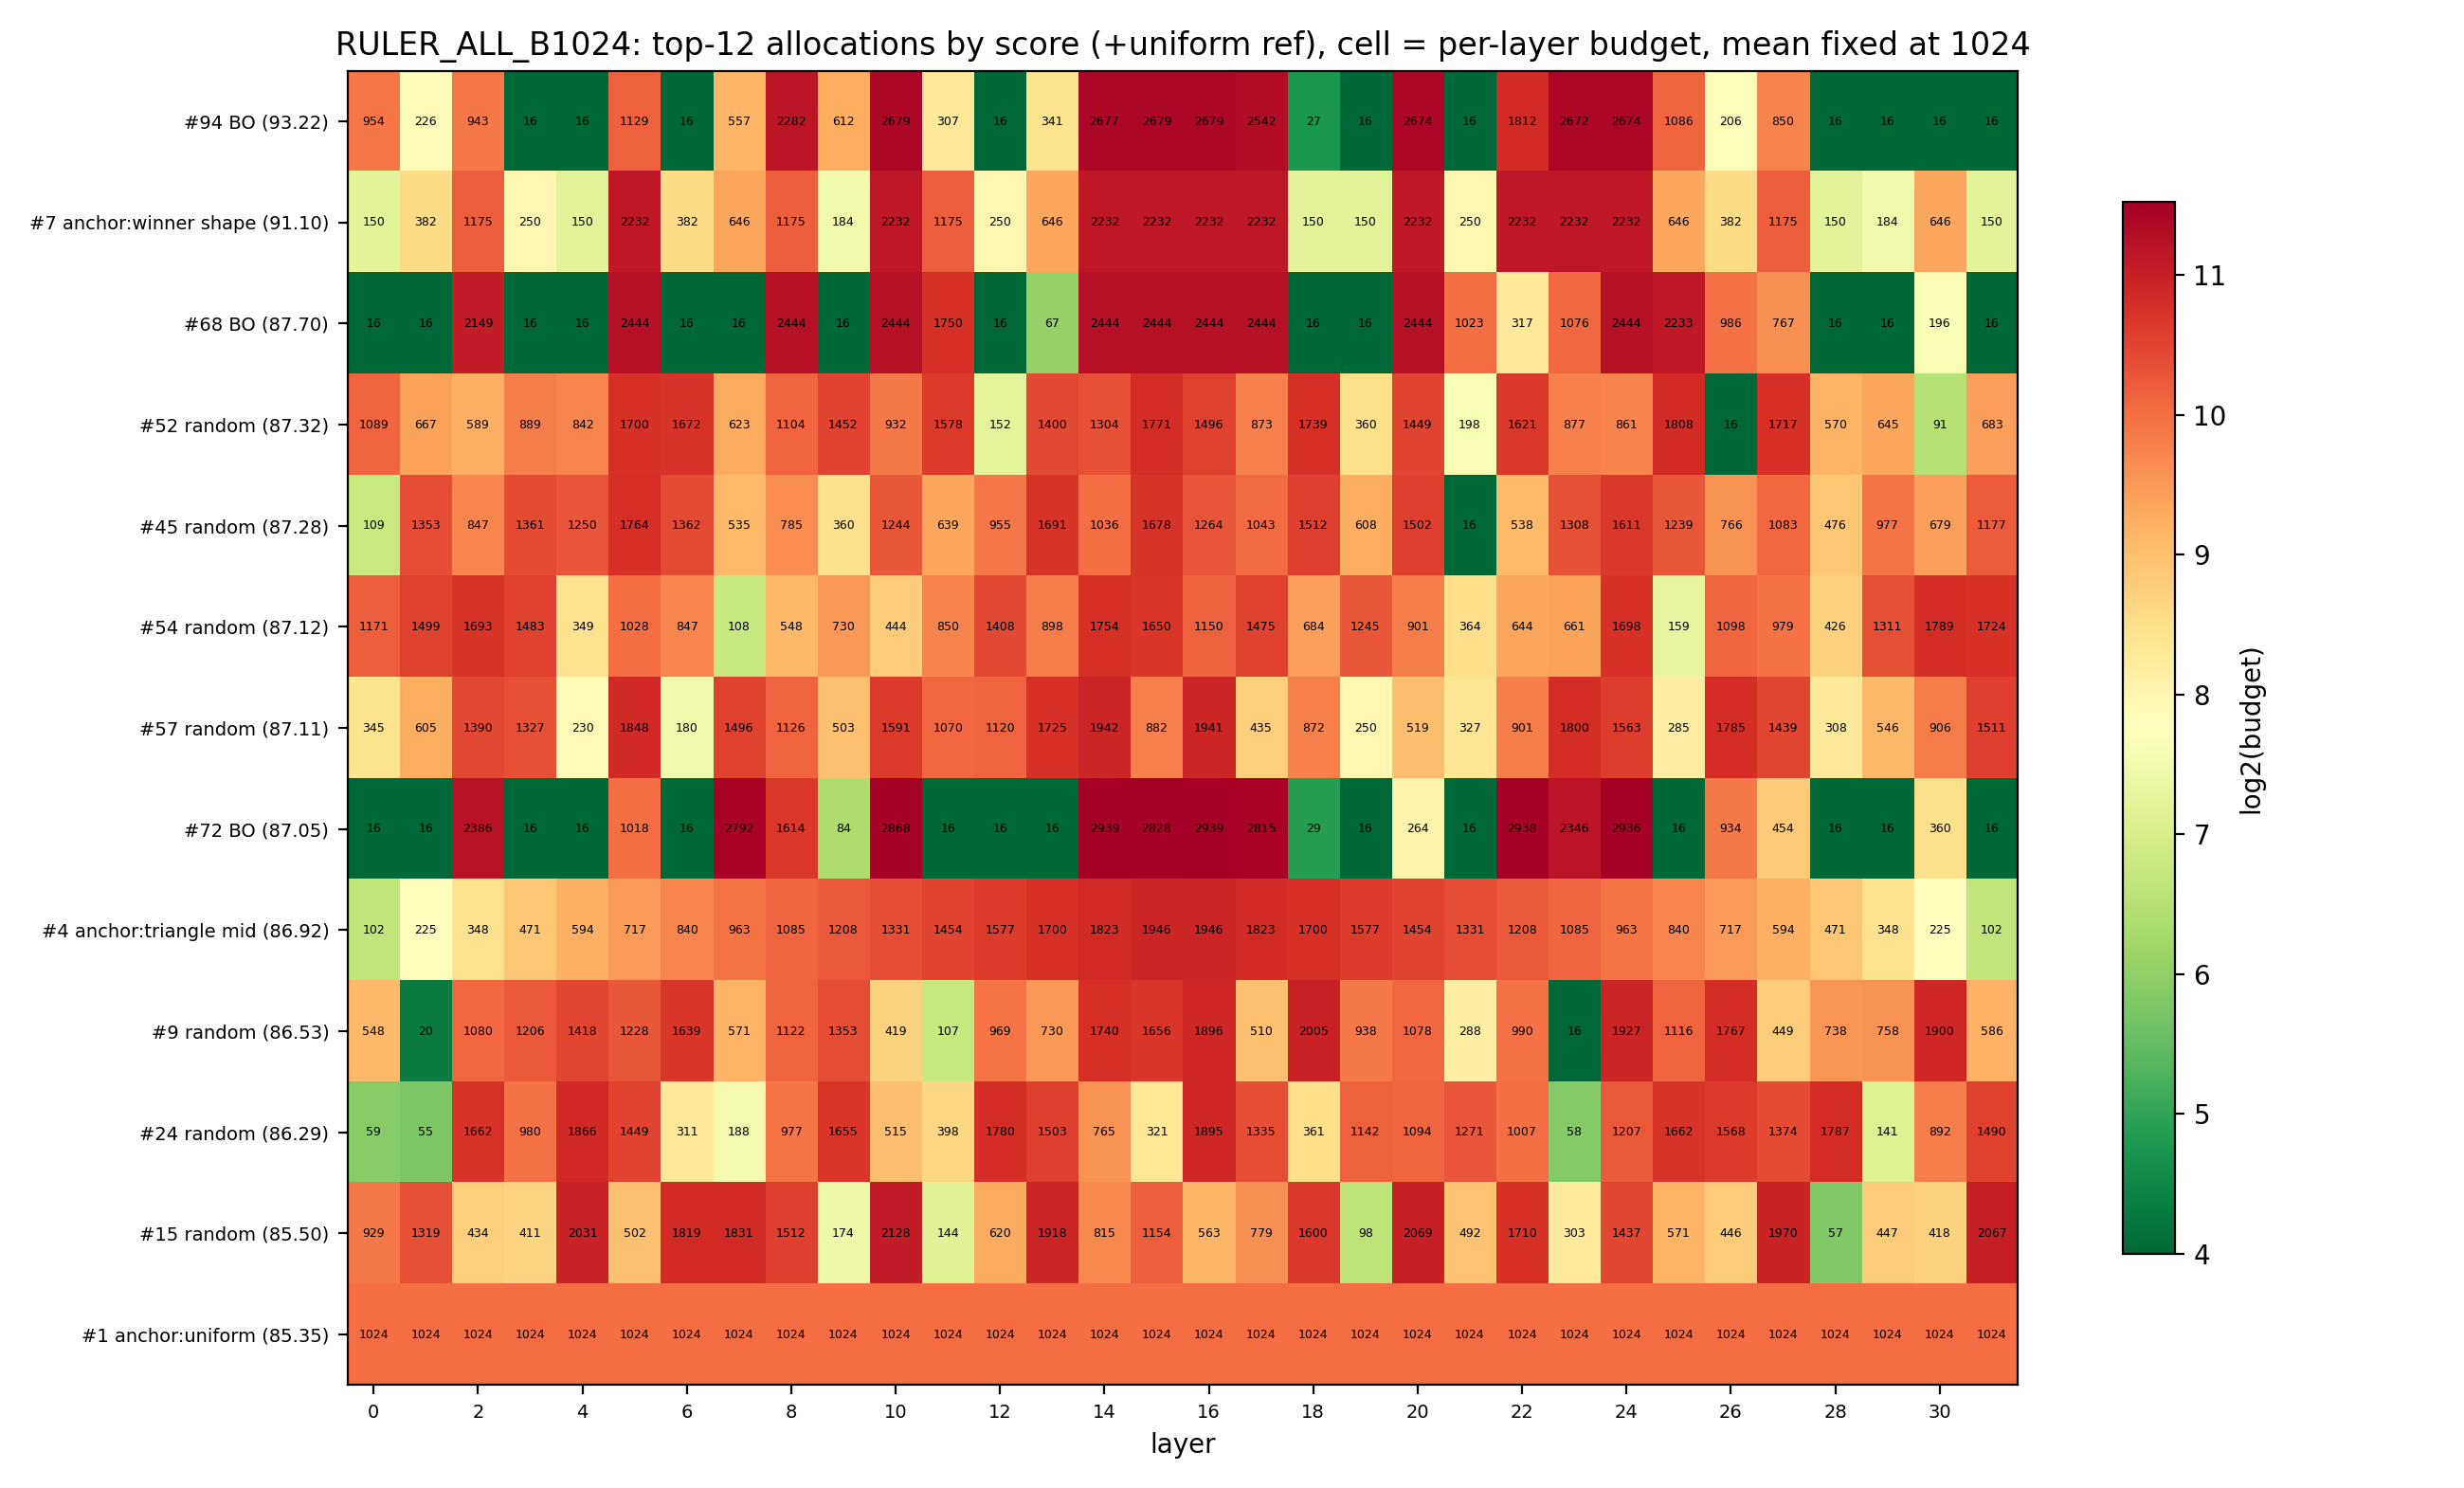
\includegraphics[width=\columnwidth]{figures/figure2_heatmap.png}
  \caption{\textbf{Floor-16 example (not used for the main results).} Per-layer budgets of five SnapKV configurations on RULER B1024, searched under the earlier floor of 16. The top BO configuration places 10 of 32 layers at 16, where only 8 tokens are selected by attention.}
  \label{fig:app-floor16}
\end{figure}


\paragraph{Controlled comparison.} Table~\ref{tab:app-floor-ablation} decodes the same rescaled SnapKV winner under both floors and evaluates both on full data. Floor 64 is better in three cells, all at B128 (by 0.37--1.10 points), the two are tied in two cells, and floor 16 is better in one (by 0.26). The differences concentrate at the lowest budget, where the floor binds most often.

\begin{table}[!htbp]
  \centering
  \scriptsize
  \setlength{\tabcolsep}{3pt}
  \begin{tabular}{@{}l r r r r@{}}
    \toprule
    Cell & Uniform & Floor 64 & Floor 16 & $\Delta$ (16$-$64) \\
    \midrule
    Code B128 & 54.81 & 55.86 & 54.76 & \textbf{$-$1.10} \\
    Code B256 & 55.67 & 57.33 & 57.30 & \textbf{$-$0.02} \\
    SingleDoc B128 & 32.97 & 33.51 & 33.14 & \textbf{$-$0.37} \\
    SingleDoc B256 & 35.25 & 34.51 & 34.77 & +0.26 \\
    MultiDoc B128 & 34.82 & 35.02 & 34.32 & \textbf{$-$0.70} \\
    MultiDoc B256 & 35.60 & 36.31 & 36.31 & +0.00 \\
    \bottomrule
  \end{tabular}
  \caption{\textbf{Same rescaled winner under floor 64 and floor 16} (SnapKV, LongBench, full data). Negative $\Delta$ (bold): floor 64 is better.}
  \label{tab:app-floor-ablation}
\end{table}


\section{Search Dynamics}
\label{app:dynamics}

Figure~\ref{fig:app-stage1} shows what the unconstrained Stage 1 search explores, for AdaKV on LongBench: every evaluated configuration and the Pareto front on the calibration score (30\% subsample). Only the front is carried to Stage 2, where it is re-evaluated on full data (Figure~\ref{fig:pareto}); many front points do not keep their advantage there.

\begin{figure*}[t]
  \centering
  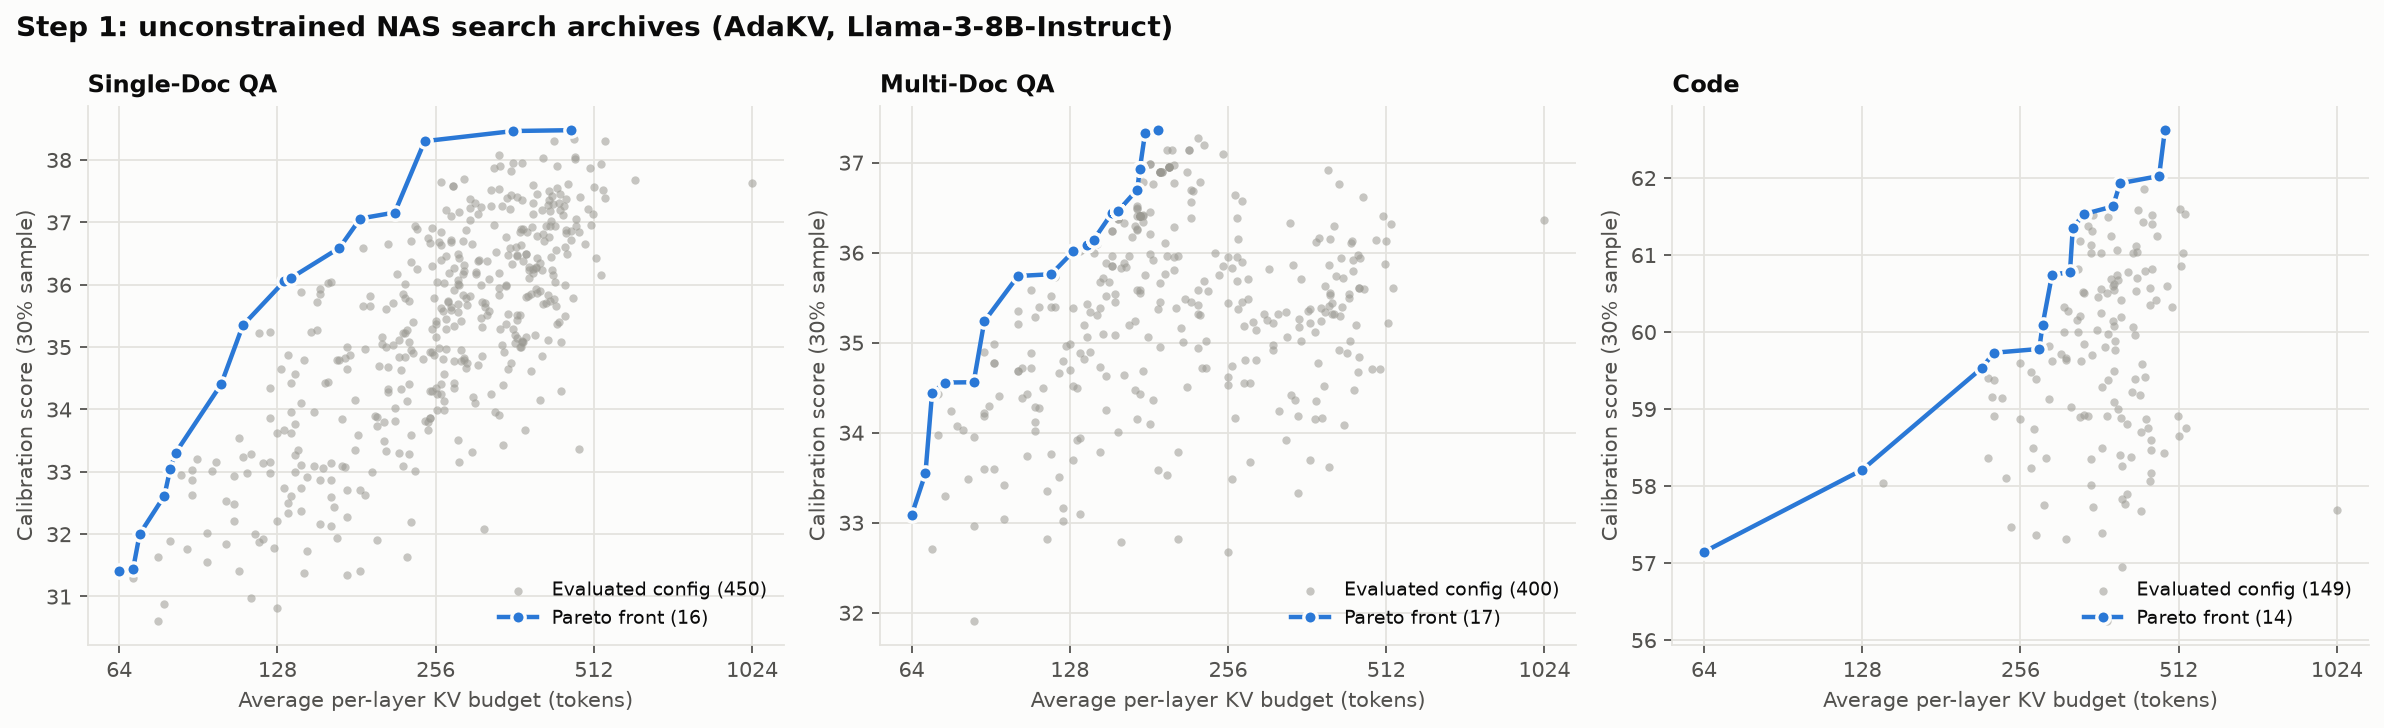
\includegraphics[width=\textwidth]{figures/adakv_stage1_archives.png}
  \caption{\textbf{Stage 1 search archives, AdaKV on LongBench (calibration scores).} Grey: every evaluated configuration; blue: the Pareto front on average budget vs.\ calibration score. ``Step 1'' in the plot title is Stage 1.}
  \label{fig:app-stage1}
\end{figure*}

Figure~\ref{fig:convergence} shows one Stage 4 search in detail: SnapKV on RULER at B1024, a cell searched under the earlier per-layer floor of 16 (Appendix~\ref{app:floor}). On RULER the calibration score tracks the full-data score (Appendix~\ref{app:calib}), so the best score found by BO is informative there; on LongBench it is not (Section~\ref{sec:which-stage}).

\begin{figure*}[t]
  \centering
  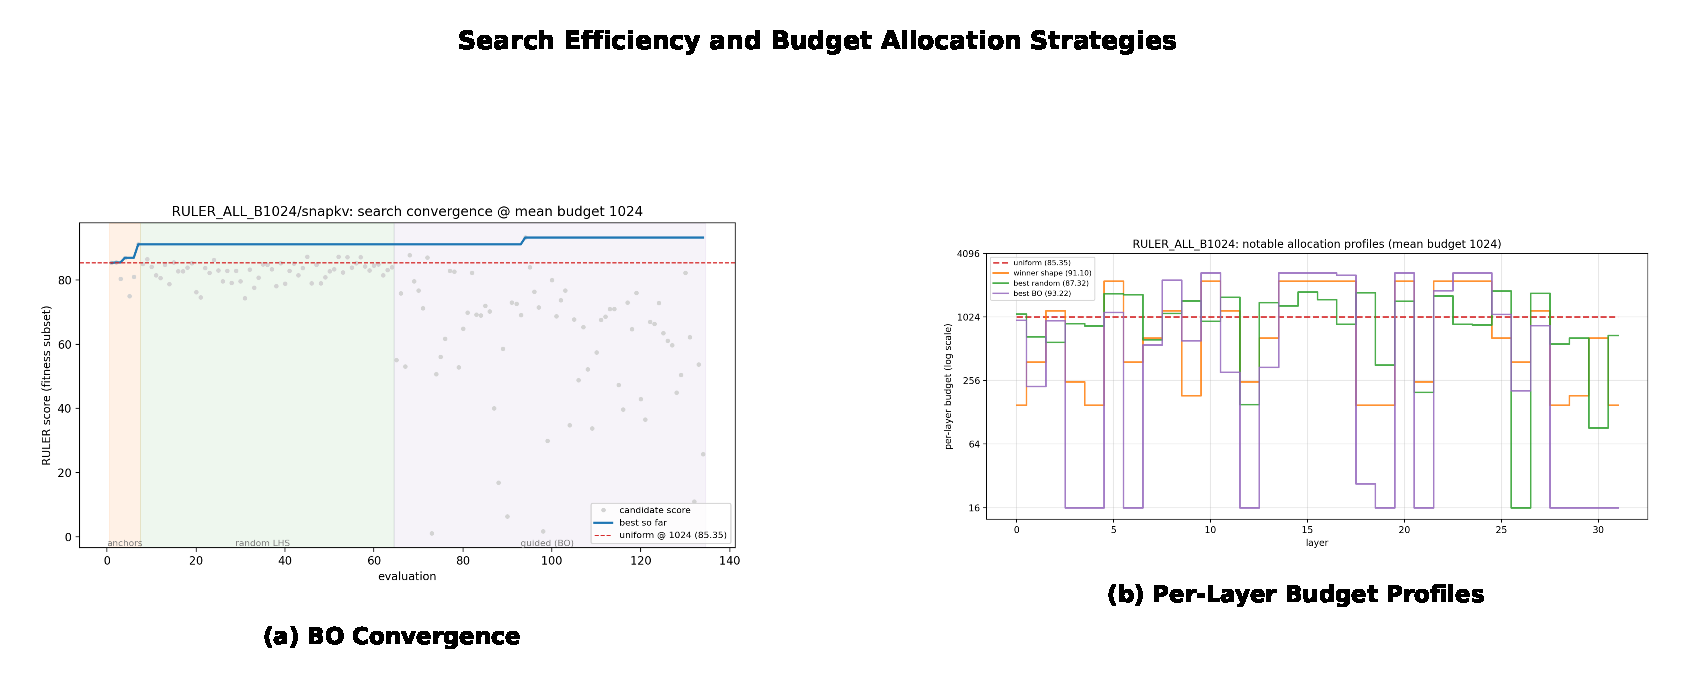
\includegraphics[width=0.95\textwidth]{figures/figure3_convergence_profiles.pdf}
  \caption{\textbf{Stage 4 search on SnapKV, RULER B1024 (floor 16).} \textit{(a)} Best calibration score found versus BO iteration. \textit{(b)} Per-layer budgets of uniform, the Winner and configurations from the Stage 4 search.}
  \label{fig:convergence}
\end{figure*}


\paragraph{Search length on LongBench.} Table~\ref{tab:app-search-curve} takes eight SnapKV Stage 4 searches and, for each, the configuration with the best calibration score among the first 64 evaluations (the initial design) and among all evaluations, both scored on full data. On average the longer search does not improve on its initial design (+0.47 against +0.72 over uniform): it changes the pick in three cells, for the better in one and for the worse in two. These are the picks calibration alone would make; NAS-refined differs because it compares several candidates of the search on full data (in Code B512 it gains +1.28). On LongBench a higher calibration score found later in the search often does not carry over to the full data (Appendix~\ref{app:calib}), which is why MOSAIC selects its final configuration on full data and keeps the Winner as a candidate.

\begin{table}[!htbp]
  \centering
  \footnotesize
  \setlength{\tabcolsep}{4pt}
  \begin{tabular}{@{}l r r r@{}}
    \toprule
    Cell & Evals & $\Delta$, first 64 & $\Delta$, all \\
    \midrule
    Code B128 & 542 & +0.91 & +1.28 \\
    Code B256 & 216 & +0.32 & +0.32 \\
    Code B512 & 148 & +1.04 & \textbf{$-$1.07} \\
    Code B1024 & 125 & +2.89 & +2.89 \\
    SingleDoc B128 & 1000 & +0.70 & +0.48 \\
    SingleDoc B256 & 501 & +0.00 & +0.00 \\
    SingleDoc B512 & 152 & \textbf{$-$0.69} & \textbf{$-$0.69} \\
    SingleDoc B1024 & 211 & +0.57 & +0.57 \\
    \textbf{Mean} &  & +0.72 & +0.47 \\
    \bottomrule
  \end{tabular}
  \caption{\textbf{Calibration-best configuration after the initial design vs.\ after the full Stage 4 search} (SnapKV, LongBench, full data). $\Delta$: gain over uniform; losses in bold.}
  \label{tab:app-search-curve}
\end{table}


\section{AdaKV Per-Layer Allocations}
\label{app:adakv-shapes}

Figure~\ref{fig:app-adakv-shapes} is the AdaKV counterpart of Figure~\ref{fig:heatmap}, drawn in the same way. AdaKV shows a weaker version of the middle-layer preference: layer 10 receives more than its uniform share in 95\% of the 19 AdaKV allocations and layers 13--16 in 68--89\%, but over the whole middle block (layers 10 and 14--20) the share is 55\%, against 65\% for SnapKV and H2O.

\begin{figure*}[t]
  \centering
  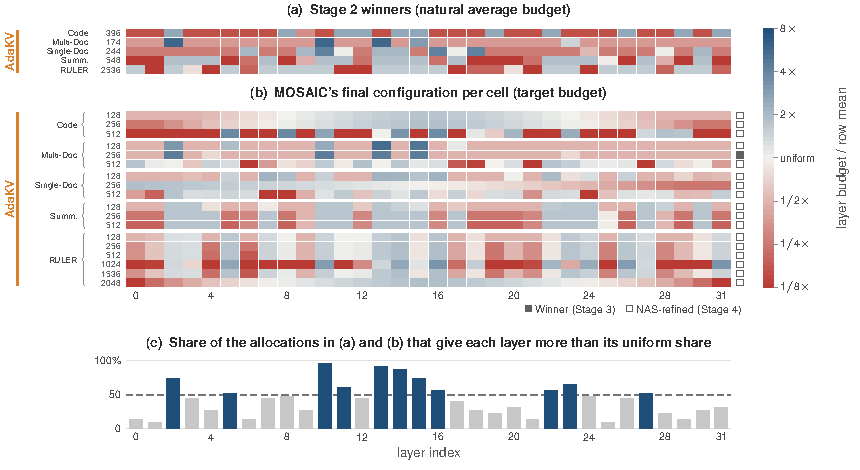
\includegraphics{figures/figure_adakv_layers.pdf}
  \caption{\textbf{AdaKV per-layer allocations}, drawn as Figure~\ref{fig:heatmap}. \textit{(a)} Stage 2 winners at their natural average budget (left). \textit{(b)} MOSAIC's final configuration for every cell (the better of Winner and NAS-refined), with the target budget on the left ($^\dagger$: searched with the earlier floor of 16) and a marker on the right for which of the two it is. \textit{(c)} For each layer, the share of the 19 allocations in (a) and (b) that give it more than its uniform share; navy bars exceed 50\%. Colour: each layer's budget divided by the row mean, on a log$_2$ scale (blue: more than the uniform share; red: less).}
  \label{fig:app-adakv-shapes}
\end{figure*}


\section{MOSAIC and EvolKV at a Glance}
\label{app:evolkv-glance}

Table~\ref{tab:app-evolkv-glance} sets MOSAIC and EvolKV \citep{yu2025evolkv} side by side. Result rows are full-data scores for SnapKV on Llama-3-8B-Instruct from Section~\ref{sec:evolkv}. Each block pairs scores with the cost of the protocol that produced them: \emph{search once} (no search at the target budget) and \emph{search at each budget}.

\begin{table*}[t]
  \centering
  \footnotesize
  \setlength{\tabcolsep}{5pt}
  \renewcommand{\arraystretch}{1.15}
  \begin{tabular}{@{} p{0.24\textwidth} p{0.32\textwidth} p{0.36\textwidth} @{}}
    \toprule
    & \textbf{EvolKV} & \textbf{MOSAIC} \\
    \midrule
    Layer budgets & one per layer, optimized block by block (4 groups of 8, earlier groups frozen) & one per layer, all 32 optimized jointly \\
    Search space of one search & 8-dimensional (one group, the other 24 layers fixed), at one budget: $\approx 2\times10^{15}$ allocations at B128, $\approx 10^{16}$ over its four searches & 32-dimensional; Stage 1: $5^{32}$ or $7^{32}$ ($\approx 10^{22}$--$10^{27}$) grid configurations across all budgets; Stage 4: $\approx 10^{69}$ allocations at B128 (${\sim}10^{53}\times$ EvolKV) to $10^{111}$ at B2048 \\
    Initial search & task score at a target average budget fixed beforehand (128) & average budget and task score as separate objectives; no target budget imposed \\
    Search output & one allocation, selected by the search fitness & a Pareto set of budget--score trade-offs, from which one anchor (the winner) is selected \\
    Reaching other budgets & rescale the allocation (expanded), or run a separate search at each budget (direct) & rescale the anchor (Stage 3), optionally refine at each budget (Stage 4) \\
    Search at a target budget starts from & the uniform allocation at that budget & the rescaled anchor, six heuristic shapes and 57 LHS points \\
    Optimizer & CMA-ES, one group at a time & classifier-guided Bayesian optimization (MLP + differential evolution) \\
    Eviction methods tested & SnapKV & SnapKV, H2O, AdaKV, L2Norm \\
    Benchmarks tested & LongBench Code, Single-Doc QA & LongBench (4 categories), RULER \\
    \midrule
    \multicolumn{3}{@{}l}{\textit{Search once: EvolKV expanded from B128 vs.\ MOSAIC Winner}} \\
    Code, B256/512/1024 & 55.99 / 56.82 / 56.42 & \textbf{57.33} / \textbf{58.16} / \textbf{58.52} \\
    Single-Doc, B256/512/1024 & \textbf{35.43} / 36.14 / 36.38 & 34.51 / \textbf{36.33} / \textbf{36.46} \\
    \multicolumn{3}{@{}l}{\textit{Search once vs.\ search at each budget: EvolKV direct vs.\ MOSAIC Winner}} \\
    Code, B128/512/1024 & 54.92 / 57.02 / 57.20 & \textbf{55.86} / \textbf{58.16} / \textbf{58.52} \\
    Single-Doc, B128/512/1024 & 33.50 / 36.28 / 36.40 & \textbf{33.51} / \textbf{36.33} / \textbf{36.46} \\
    One-time cost (A100) & 12.7 (Code), 5.2 (Single-Doc) GPU-h & Code: 8.0 GPU-h for Stage 2, Stage 1 logs lost; Single-Doc: 20.1 GPU-h \\
    \midrule
    \multicolumn{3}{@{}l}{\textit{Search at each budget, MOSAIC capped at EvolKV's per-cell cost: EvolKV direct vs.\ MOSAIC NAS-refined}} \\
    Code, B128/512/1024 & 54.92 / 57.02 / 57.20 & \textbf{$\geq$55.73} / \textbf{58.01} / \textbf{58.91} \\
    Single-Doc, B128/512/1024 & 33.50 / \textbf{36.28} / 36.40 & \textbf{33.67} / 35.61 / \textbf{37.01} \\
    Cost, 6 cells (A100) & 53.7 GPU-h & 47.2 GPU-h capped (84.9 as run), plus the one-time Stages 1--2 that seed it \\
    \bottomrule
  \end{tabular}
  \caption{\textbf{EvolKV vs.\ MOSAIC.} Bold marks the better score within each block. Costs are measured on the same hardware and harness (Appendix~\ref{app:cost}). MOSAIC's search-once Winner wins on Code but needs a costlier one-time search; with each Stage 4 search truncated to EvolKV's per-cell cost, NAS-refined wins 5 of 6 cells (Table~\ref{tab:app-capped}; $\geq$: lower bound), a comparison that excludes MOSAIC's one-time Stages 1--2.}
  \label{tab:app-evolkv-glance}
\end{table*}


\section{Reproducibility Details}
\label{app:repro}

\paragraph{Budget decoding.} Stage 1 maps each coordinate $x_i \in [0,1]$ of a configuration to a discrete per-layer budget by equal-width bins over a grid $G$, $b_i = G[\min(\lfloor x_i |G| \rfloor, |G|-1)]$: seven levels from 64 to 4096 on RULER, for L2Norm and for H2O on Code, and five from 64 to 1024 for the other LongBench runs (SnapKV, AdaKV, H2O); for SnapKV Code, whose Stage 1 log was lost, the 1024 cap is inferred from its winner. The grid limits only Stage 1: Stages 3 and 4 decode continuously within $[64, 4096]$ for every run, so a winner found under the 1024 cap can receive larger per-layer budgets after rescaling. The total cache, and hence memory, is fixed by the average budget $B$, so this only redistributes budget across layers; LongBench inputs (up to 7{,}500 tokens after truncation) are longer than the 4096 cap, so a layer's extra budget is spent on retaining more tokens. Stages 3 and 4 use a continuous decoder that fixes the mean at the target $B$. With total $T = 32B$ and weights $w_i = \max(x_i, 10^{-6})$, it sets $b_i = R\,w_i / \sum_{j \in F} w_j$ for the free layers $F$, where $R$ is $T$ minus the budget of the clamped layers. Layers above the cap of 4096 are clamped first; only when none exceeds it are layers below the floor clamped; clamped layers stay clamped, and the step repeats until no bound is violated (at most 32 passes). The surplus or deficit is therefore redistributed in proportion to $w_i$ over the free layers. Budgets are then rounded down, and the remaining tokens go one each to the free layers with the largest fractional parts; ties go to the lower layer index (stable sort), so $\sum_i b_i = T$ exactly whenever $32 \cdot 64 \le T \le 32 \cdot 4096$. \emph{Search-space size.} The Stage 1 grid holds $|G|^{32}$ configurations. At a fixed budget $B$, the number of integer allocations $b \in [64, 4096]^{32}$ with $\sum_i b_i = 32B$ follows by inclusion--exclusion over the cap, $\sum_k (-1)^k {32 \choose k}{S - 4033k + 31 \choose 31}$ with $S = 32(B - 64)$: about $10^{69}$, $10^{84}$, $10^{95}$, $10^{105}$ and $10^{111}$ at B128, B256, B512, B1024 and B2048; at B64 the floor leaves only the uniform allocation. For EvolKV we count, per search, the allocations of one 8-layer group in $[64, 4096]^8$ whose mean equals the target $c$, where its CacheScore term peaks, with the other groups fixed (the same formula with 8 layers): about $2\times10^{15}$ at $c = 128$, so its four searches cover about $10^{16}$, against $10^{69}$ for one joint MOSAIC search at B128, a factor of about $10^{53}$.

\paragraph{Rescaling the Stage 2 winner.} A winner with per-layer budgets $w_i$ is mapped to $x_i = 0.05 + 0.9\,w_i / \max_j w_j$ and decoded at each target $B$ as above. This keeps the order of the layers and the shape of the allocation, but it is an affine map rather than an exact proportional one: ratios between layers are compressed (a layer at the winner's minimum receives at least $0.05/0.95$ of the largest layer's budget). The same mapping seeds the winner into the Stage 4 search.

\paragraph{Per-layer floor and cap.} The cap is 4096 in every run. The floor is 64 except in runs launched under an earlier default of 16: RULER B1024--B2048 for SnapKV, H2O and AdaKV (at B1536--B2048 no SnapKV or H2O final configuration reaches it), the rescaled SnapKV RULER winners at B64 and B512, and AdaKV RULER B64. Every Llama LongBench cell and every L2Norm cell uses floor 64; the Mistral SnapKV, H2O and AdaKV RULER runs use floor 16 throughout. Table~\ref{tab:app-floor} reports how often the floor binds.

\paragraph{Initial designs.} Stage 1 starts from the uniform allocation at every grid level (5 or 7 points, $x_i$ at the bin centres) followed by Latin Hypercube points (59 or 57) drawn with seed 43. Stage 4 rows 0--63 are, in order: uniform ($x_i = 0.5$); five heuristic shapes, namely an ascending ramp ($x$ linear from 0.05 to 0.95 over layers 0--31), its reverse, a middle-heavy triangle (0.05 to 0.95 over layers 0--15, back to 0.05 over 16--31), its complement $1-x$ (edge-heavy), and an alternating pattern $(0.15, 0.85, \dots)$; the rescaled Stage 2 winner, $x_i = 0.05 + 0.9\,w_i/\max_j w_j$; and 57 Latin Hypercube points (seed 43). Calibration subsets use a separate seed (42, below).

\paragraph{Surrogate.} The rank-1 classifier is a scikit-learn \texttt{MLPClassifier} with hidden layers (32, 32) and library defaults otherwise (ReLU, Adam, 200 iterations); proposals maximize its rank-1 probability with SciPy's \texttt{differential\_evolution} at library defaults (\texttt{best1bin}, population 15, up to 1000 generations, polishing on). Neither is seeded, so reruns are not bit-identical.

\paragraph{Stopping rules.} The evaluation cap is 1000 (64 initial + 936 guided). H2O LongBench Stage 4 and SnapKV Summarization Stage 4 use a cap of 200. Other SnapKV LongBench Stage 4 runs were stopped by a saturation watchdog: a run ends when the best calibration score has not improved over the last 40 rows, after at least 60 rows beyond the initial design. Two kept runs, Code B128 and Multi-Doc QA B256, were stopped by an earlier watchdog with a patience of 15 rows after 20, and Single-Doc and Multi-Doc QA B128 reached the 1000 cap. SnapKV and H2O RULER Stage 4 runs stop after 40 evaluations without a new best (counted from the later of the best row and row 64) or at 160 rows. AdaKV searches were stopped by hand once the archive had settled or after a crash; the Mistral AdaKV RULER searches at B1024--B2048 were stopped after only 3--26 evaluations, so their results are close to the initial design. Stage 1 runs were stopped by hand; H2O RULER Stage 1 used at least 198 evaluations, 40 without a new best shaped configuration, and a cap of 350. L2Norm's stopping rule is not recorded in the files available to us.

\paragraph{Candidate provenance.} Stage 2 re-evaluates every distinct rank-1 configuration of the Stage 1 archive on full data, and the winner is the non-uniform configuration with the highest full-data score. The RULER winners were taken by calibration score instead: for SnapKV this is also the full-data best, and for H2O only the four top calibration-ranked configurations were re-evaluated, whose full-data ranking equals the calibration ranking. Stage 4 re-evaluates, besides uniform and the Winner, the calibration-best row of each group: heuristic shapes (rows 1--5), Latin Hypercube points (rows 7--63) and guided proposals (rows 64 and later); NAS-refined is the best of these three on full data. Earlier RULER cells used fewer candidates: SnapKV and H2O B1024 and H2O B1536--B2048 re-evaluated uniform, the best of rows 1--6, the best LHS point and the best row overall; SnapKV B1536--B2048 re-evaluated uniform, the Winner and the best LHS point only. If a run was restarted, the restart's initial design was appended after row 63 and counts as guided rows.

\paragraph{Unavailable records.} The Code Stage 1 archives and logs (SnapKV and H2O) were lost; only their Stage 2 re-evaluations survive. AdaKV RULER Stage 1 timings, the SnapKV Multi-Doc QA Stage 1 timing, and L2Norm search timings are not available.

\paragraph{EvolKV expansion.} Following EvolKV's budget completion rule \citep{yu2025evolkv}, an allocation $k_i$ found at budget 128 is expanded to target $B$ by $b_i = k_i\,T / \sum_j k_j$, rounded with the largest-remainder method so that the mean is exactly $B$, and clipped to $[64, 4096]$ (neither bound binds for B256--B1024).

\paragraph{Evaluation settings.} Llama-3-8B-Instruct in float16, greedy decoding (one beam). LongBench uses the official prompts and chat template, middle truncation of inputs longer than 7{,}500 tokens (the first and last 3{,}750 tokens are kept), the official per-dataset output lengths (32--512 tokens) and the official metrics (F1 for QA, ROUGE-L for summarization, edit similarity for code). RULER uses its 11 subtasks at 4K context with string-match accuracy. SnapKV and H2O keep a fixed recent window of 8 tokens; SnapKV pools observation-window scores with a max-pool of kernel size 7. Calibration subsets are drawn per dataset with Python's \texttt{random.Random(42).sample} at the stated ratio, and the same seed is used throughout. All four methods use FlashAttention-2 for attention.

\paragraph{Hardware.} Searches and evaluations ran on four servers: SnapKV, H2O and AdaKV on NVIDIA A100 GPUs (the EvolKV comparison on the same A100-40GB machine and harness as MOSAIC), AdaKV additionally on RTX A6000 GPUs, and L2Norm on H100 GPUs. The Mistral-7B-Instruct-v0.2 L2Norm searches ran on H100 GPUs with a 30\% calibration subset in every stage, and the Mistral SnapKV, H2O and AdaKV RULER searches on A100 GPUs with a 10\% subset.
